\documentclass[12pt,a4paper]{book}

\usepackage{longtable}
\usepackage{caption,subcaption}
\usepackage{amsmath}
\usepackage{amsthm}
\usepackage{amsfonts}
\usepackage{amssymb}
\usepackage{multirow}
\usepackage{multicol}
\usepackage[spanish]{babel}
\usepackage{graphicx}
\usepackage[table]{xcolor}
\usepackage{wrapfig}
\usepackage{float} 
\usepackage[margin=3.5cm]{geometry}
\hyphenation{Re-fe-ren-cias}
\usepackage{fancyhdr}
\graphicspath{ {figures/} }
%\usepackage{color}              
% For creating coloured text and background
\usepackage[hyphens]{url}            
% For preventing long urls from going past margin
\usepackage[hidelinks]{hyperref}            
% For creating hyperlinks in cross references
\columnsep 0.8 cm
\pagestyle{plain}
\newtheorem{teorema}{Teorema}
\fancyfoot{}


\usepackage{listings}
\usepackage{color}

\begin{document}
	\renewcommand{\tablename}{Tabla}
	\renewcommand{\refname}{Referencias bibliográficas.}
	
	
\begin{titlepage}
	\newlength{\centeroffset}
	\setlength{\centeroffset}{-0.5\oddsidemargin}
	\addtolength{\centeroffset}{0.5\evensidemargin}
	\thispagestyle{empty}
	
	\vspace{3cm}
	
	\begin{figure}[h!]
		\centering
		
\includegraphics[width=1\linewidth]{figures/logo}
		\label{fig:logo}
	\end{figure}
	
	%\thispagestyle{empty}
	\vspace{0.5cm}
	\noindent\hspace*{\centeroffset}\begin{minipage}{\textwidth}
		
		\centering
		
		\textsc{ \Large TRABAJO FIN DE GRADO\\[0.2cm]}
		\textsc{ INGENIERÍA EN INFORMÁTICA}\\[1cm]
		% Upper part of the page
		% 
		% Title
		{\Huge\bfseries Desarrollo de un sistema de alerta temprana financiera basada en aprendizaje automático avanzado\\
		}
		\noindent\rule[-1ex]{\textwidth}{3pt}\\[3.5ex]
	\end{minipage}
	

\vspace{1cm}
	\noindent\hspace*{\centeroffset}\begin{minipage}{\textwidth}
		\centering
		
		\textbf{Autor}\\ {Rafael Vázquez Conejo}\\[2.5ex]
		\textbf{Director}\\
		{Salvador García López}\\[2cm]

	\end{minipage}

		

	
	
\vspace{1cm}
\begin{figure}[h!]
	\centering
	
\includegraphics[width=0.3\linewidth]{figures/logo2}
	\label{fig:logo2}
\end{figure}


\noindent\hspace*{\centeroffset}\begin{minipage}{\textwidth}
	\centering
\textsc{Escuela Técnica Superior de Ingenierías Informática y de Telecomunicación}\\
\textsc{---}\\
Granada, julio de 2022
\end{minipage}


\end{titlepage}
	
	\clearpage\hbox{}\thispagestyle{empty}\newpage
	
	\tableofcontents
	
	\vspace{1cm}
	
	\newpage
	
	\thispagestyle{empty}
	
	
	
	\chapter{Introducción}
Este documento recoge el informe obtenido con la realización del trabajo final de la asignatura \textit{Introducción a la Ciencia de Datos}. Este consiste en la realización de un análisis exploratorio de los datos pertenecientes a dos \textit{dataset} distintos, con la intención de comprender y determinar información importante sobre las variables que forman a cada conjunto de datos. Tras ello, dependiendo del dataset, se generarán diversos modelos de clasificación o regresión.\cite{dataMining} \\

El primer dataset tratado es el \textbf{California}, sobre el que se plantea un problema de regresión y la búsqueda de desarrollar diversos modelos óptimos de regresión lineal simple y múltiple, modelos de regresión basados en K-NN (K Nearest Neighbour) y modelos de regresión no lineales.
\textbf{Bupa} es el segundo dataset, el cual plantea un problema de clasificación que será abordado con modelos de clasificación basados en KNN, modelos basados en LDA y modelos basados en QDA.
	\chapter{Análisis Exploratorio de los Datos (EDA). Dataset de regresión: California}

\section{Descripción del dataset: California}
El dataset \textbf{California} contiene información relativa a viviendas de California, formada por datos extraídos del censo de Estados Unidos del 1990, cuya variable objetivo es el valor medio de la vivienda para diferentes distritos de California, información expresada en cientos de miles de dólares (\$100,000). \\
Cada fila de este conjunto de datos representa un grupo de bloques censales, siendo esta la unidad geográfica más pequeña utilizada por La Oficina del Censo de EE.UU. para publicar sus datos (generalmente un grupo de bloques lo forma una población de 600 a 3.000 personas). \cite{3}

\vspace{0.5cm}
Este dataset consta de 8 variables independientes y una variable dependiente, siendo todos los datos numéricos. Se recoge en total 20640 muestras que representan diferentes bloques censales.\\
Se presentan a continuación las variables independientes:
\begin{itemize}
	\item \textbf{Longitude}: Variable numérica real que refleja la longitud geográfica del grupo de bloques censal.
	\item \textbf{Latitude}: Variable numérica real que refleja la latitud geográfica del grupo de bloques censal.
	\item \textbf{HousingMedianAge}: Variable numérica entera que refleja la media de antigüedad de una casa en un grupo de bloques.
	\item \textbf{TotalRooms}: Variable numérica entera que refleja la cantidad total de habitaciones por hogar.
	\item \textbf{TotalBedrooms}: Variable numérica entera que refleja la cantidad total de dormitorios por hogar.
	\item \textbf{Population}: Variable numérica entera que refleja la cantidad de personas que residen en un grupo de bloques.
	\item \textbf{Households}: Variable numérica entera que refleja la cantidad de hogares en un grupo de bloques.
	\item \textbf{MedianIncome}: Variable numérica real que refleja el valor medio de los ingresos de cada hogar de un grupo de bloques (medido en decenas de miles de dolares estadounidenses).
\end{itemize}
La variable dependiente es \textbf{MedianHouseValue}, un valor numérico entero que representa el precio medio asociado al valor de una casa en cada distrito de California. \cite{4}




\section{Planteamiento de hipótesis}
\begin{itemize}
	\item California posee una amplia zona de costa permitiendo las variables de latitud y longitud determinar la cercanía de cada grupo de viviendas al mar. ¿Cómo de importante es la localización de la vivienda a la hora de determinar su precio?
	
	\item En ocasiones zonas con menos densidad de población suele estar relacionado con poblaciones más privilegiadas, ¿el precio de la vivienda tendrá una alta relación con la densidad de la población?
	
	\item La variable MedianIncome indica los ingresos medios de los hogares, ¿posee esta una fuerte relación positiva con el valor de la vivienda?
	
	\item Un factor interesante de estudio es la antigüedad de la vivienda, lo esperable sería que una casa nueva tuviera mayor precio que una antigua. Sin embargo, puede que la localización de la vivienda afecte a esta variable y esta premisa no se cumpla.
\end{itemize}








\section{Procesamiento de los datos}
Introducidos los diferentes atributos que constituyen este dataset, el siguiente paso pretende un análisis en detalle de la información contenida en dicho dataset con el objetivo de conocer y determinar cualquier característica de los datos que facilite el posterior desarrollo de modelos predictivos. \\

El primer paso es la búsqueda de valores perdidos dentro de los datos, concluyendo en que este dataset no posee ningún Missing value.
También se determina que no hay ninguna muestra duplicada.


\subsection{Análisis de las variables}
Para un mejor análisis del comportamientos de las diferentes variables, se calculan diversas medidas de posición: la media aritmética, mediana, primer y tercer cuartil, valores máximos y mínimos de cada variable. También se estudia la dispersión de las distribuciones mediante el calculo  de la desviación típica, mientras que la normalidad de los datos se estudia con los coeficientes de Skewness y Kurtosis.\\



Se estudia cada variable en detalle mediante el calculo de las medidas previamente mencionadas. Dicho estudio es acompañado con una serie de representaciones gráficas que facilite la comprensión de los datos:

\begin{itemize}
	\item \textbf{Longitude}
			\begin{table}[h!]
				\centering
				\begin{tabular}{ll}
					& Longitude   \\
					Valor mínimo            & -124.3      \\
					Primer cuartil          & -121.8      \\
					Mediana                 & -118.5      \\
					Media                   & -119.6      \\
					Tercer cuartil          & -118.0      \\
					Valor máximo            & -114.3      \\ \hline
					Desviación estandar     & 2.003532    \\ \hline
					Coeficiente de skewness & -0.29777956 \\
					Coeficiente de Kurtosis & 1.669879   
				\end{tabular}
			\end{table}

Los estadísticos resultantes nos muestran una distribución con una medida de asimetria muy cercana al valor cero, lo que nos indica que la distribución de esta se aproxima a una distribución normal, pero con cierta dispersión de los datos a la derecha, hecho que claramente se refleja con un valor de la media muy cercano al valor del tercer cuartil.
Un coeficiente de Kurtosis tan cercano a cero nos indica que no se presenta dispersión de los valores respecto al centro de densidad de la distribución.

Se estudia de forma gráfica estos resultados por medio de un diagrama de cajas:

\begin{figure}[h!]
	\centering
	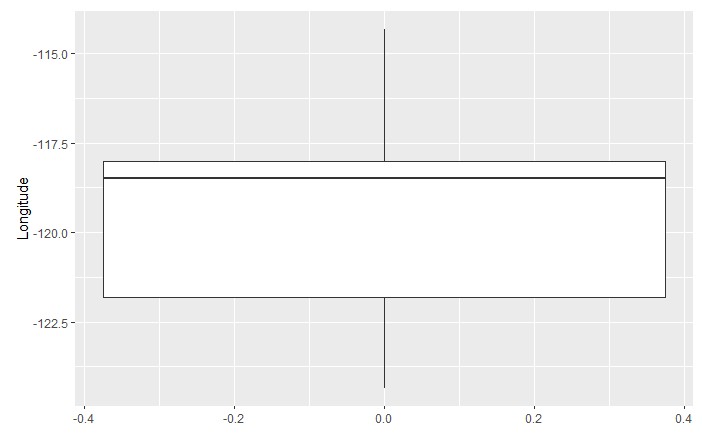
\includegraphics[width=0.7\linewidth]{figures/eda_box_1}
	\caption{Diagrama de cajas Longitude}
	\label{fig:edabox1}
\end{figure}

\newpage
Efectivamente el diagrama de cajas nos muestra que los datos se concentran en una región central densa, sin presencia de outliers.\\

Observemos la distribución de los valores en más detalle en un histograma:


\begin{figure}[h!]
	\centering
	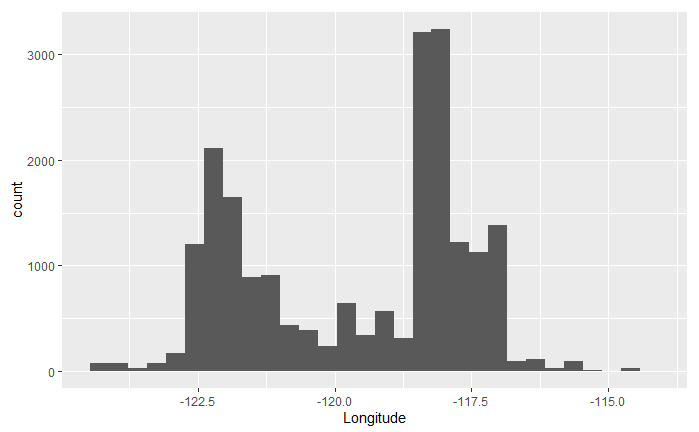
\includegraphics[width=0.7\linewidth]{figures/eda_hist_1}
	\caption{Histograma Longitude}
	\label{fig:edahist1}
\end{figure}




\newpage
	\item \textbf{Latitude}: 
	\begin{table}[h!]
		\centering
		\begin{tabular}{ll}
			& Latitude   \\
			Valor mínimo            & 32.54      \\
			Primer cuartil          & 33.93      \\
			Mediana                 & 34.26      \\
			Media                   & 35.63      \\
			Tercer cuartil          & 37.71      \\
			Valor máximo            & 41.95      \\ \hline
			Desviación estandar     & 2.135952   \\ \hline
			Coeficiente de skewness & 0.46591914 \\
			Coeficiente de Kurtosis & 1.882220  
		\end{tabular}
	\end{table}

En este caso los datos presentan una leve dispersión a la derecha, detalle que se confirma al observar una media cercana al valor del primer cuartil. De nuevo no se presenta dispersion de los datos respecto de su centro, por lo que será poco probable la existencia de outliers. \\

Se complementa este estudio con la representación gráfica de esta variable mediante un diagrama de cajas y un histograma

\begin{figure}[h!]
	\centering
	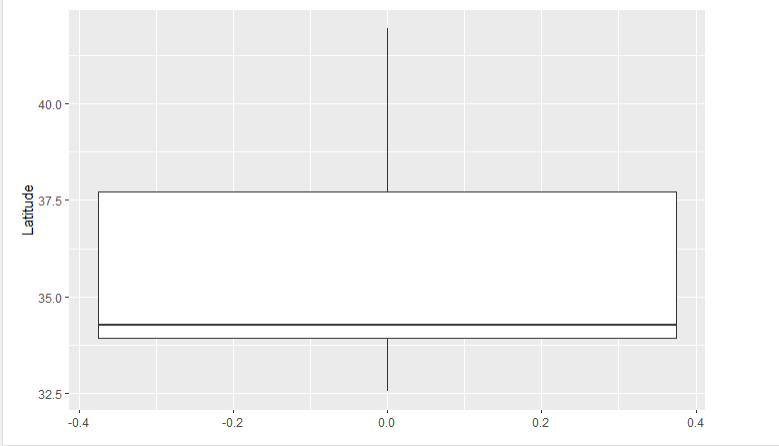
\includegraphics[width=0.7\linewidth]{figures/eda_box_2}
	\caption{Diagrama de cajas Latitude}
	\label{fig:edabox2}
\end{figure}
\newpage
\begin{figure}[h!]
	\centering
	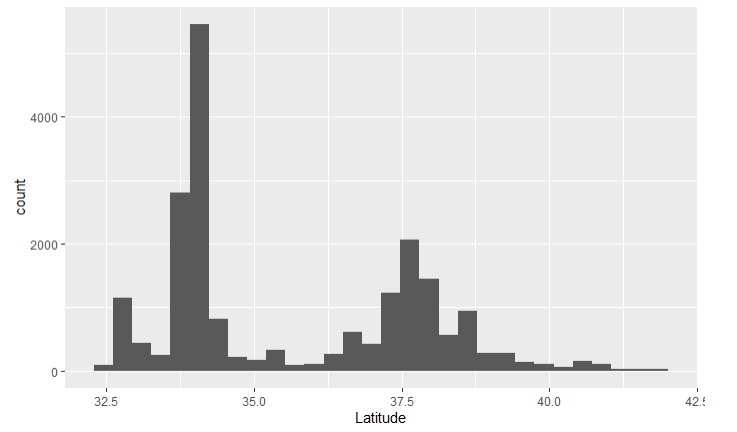
\includegraphics[width=0.7\linewidth]{figures/eda_hist_2}
	\caption{Histograma Latitude}
	\label{fig:edahist2}
\end{figure}

Se confirma una distribución concentrada de los datos levemente desplazada a valores situados a la izquierda. \\ 


	
	\item \textbf{HousingMedianAge}: 
	\begin{table}[h!]
		\centering
		\begin{tabular}{ll}
			& HousingMedianAge \\
			Valor mínimo            & 1.00             \\
			Primer cuartil          & 18.00            \\
			Mediana                 & 29.00            \\
			Media                   & 28.64            \\
			Tercer cuartil          & 37.00            \\
			Valor máximo            & 52.00            \\ \hline
			Desviación estandar     & 12.585558        \\ \hline
			Coeficiente de skewness & 0.06032625       \\
			Coeficiente de Kurtosis & 2.199274        
		\end{tabular}
	\end{table}

Los resultados estadísticos describen una variable con una región central muy densa y con una muy leve dispersión de los datos respecto a esta región central, descartando nuevamente la presencia de outliers.

Se complementa este estudio con la representación gráfica de esta variable mediante un diagrama de cajas y un histograma:
\newpage
\begin{figure}[h!]
	\centering
	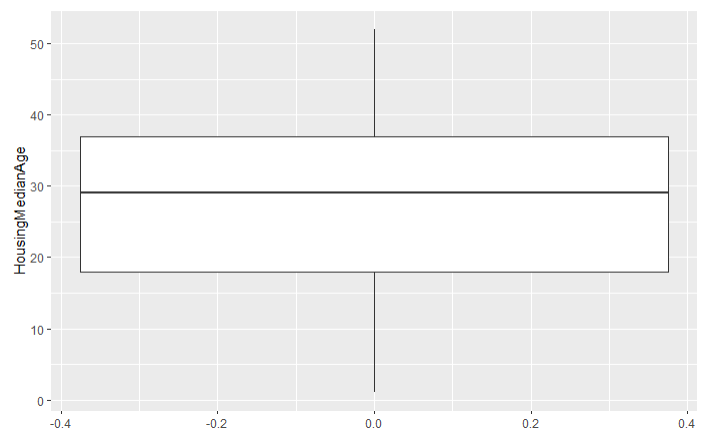
\includegraphics[width=0.7\linewidth]{figures/eda_box_3}
	\caption{Diagrama de cajas HousingMedianAge}
	\label{fig:edabox3}
\end{figure}
\begin{figure}[h!]
	\centering
	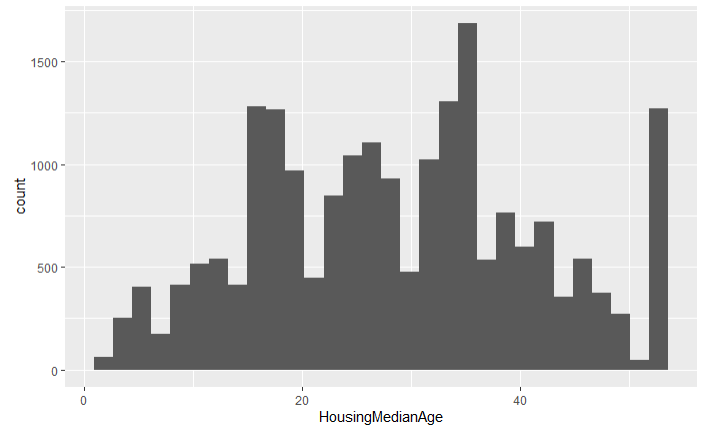
\includegraphics[width=0.7\linewidth]{figures/eda_hist_3}
	\caption{Histograma HousingMedianAge}
	\label{fig:edahist3}
\end{figure}

Se emplea el test de Shapiro-Wilk para confirmar que no se supera el nivel mínimo de significancia, y por tanto no es una distribución normal.

	
	\item \textbf{TotalRooms}: 
	\begin{table}[h!]
		\centering
		\begin{tabular}{ll}
			& TotalRooms  \\
			Valor mínimo            & 2           \\
			Primer cuartil          & 1448        \\
			Mediana                 & 2127        \\
			Media                   & 2636        \\
			Tercer cuartil          & 3148        \\
			Valor máximo            & 39320       \\ \hline
			Desviación estandar     & 2181.615252 \\ \hline
			Coeficiente de skewness & 4.14704204  \\
			Coeficiente de Kurtosis & 35.622732  
		\end{tabular}
	\end{table}


Los resultados estadísticos hacen referencia a una distribución desplazada a la izquierda. El coeficiente de Kurtosis obtenido se traduce en una amplia dispersión de los datos respecto al centro de distribución de estos, siendo en este caso, a diferencia de los anteriores, muy probable la existencia de outliers situados a la derecha.

Se complementa este estudio con la representación gráfica de esta variable mediante un diagrama de cajas y un histograma

\begin{figure}[h!]
	\centering
	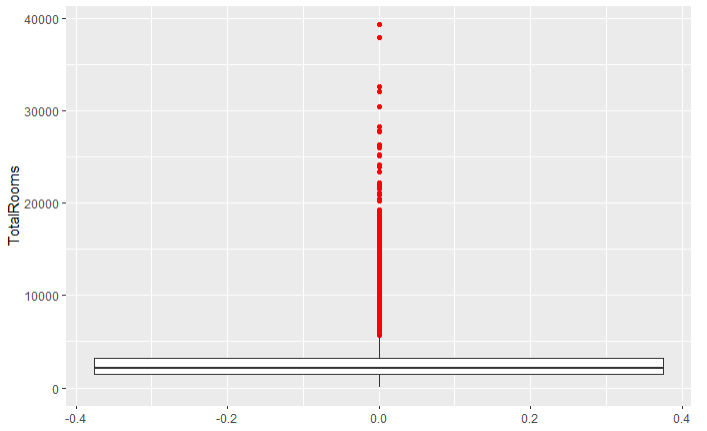
\includegraphics[width=0.7\linewidth]{figures/eda_box_4}
	\caption{Diagrama de cajas TotalRooms}
	\label{fig:edabox4}
\end{figure}
\begin{figure}[h!]
	\centering
	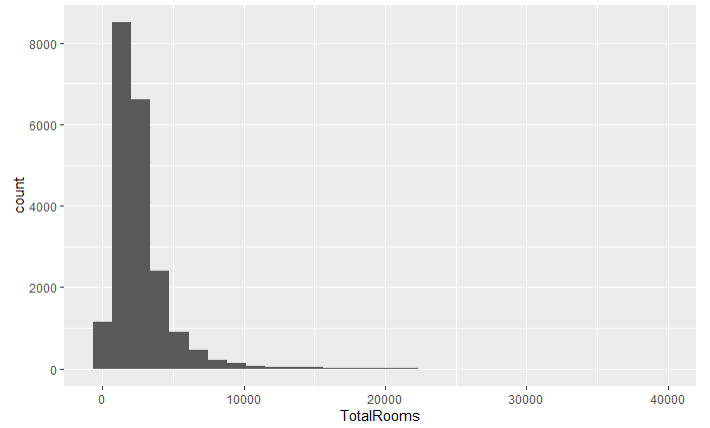
\includegraphics[width=0.7\linewidth]{figures/eda_hist_4}
	\caption{Histograma TotalRooms}
	\label{fig:edahist4}
\end{figure}


	\newpage
	\item \textbf{TotalBedrooms}: 
	\begin{table}[h!]
		\centering
		\begin{tabular}{ll}
			& TotalBedrooms \\
			Valor mínimo            & 1.0           \\
			Primer cuartil          & 295.0         \\
			Mediana                 & 435.0         \\
			Media                   & 537.9         \\
			Tercer cuartil          & 647.0         \\
			Valor máximo            & 6445.0        \\ \hline
			Desviación estandar     & 421.247906    \\ \hline
			Coeficiente de skewness & 3.45282180    \\
			Coeficiente de Kurtosis & 24.917894    
		\end{tabular}
	\end{table}

Se presenta un caso similar al anterior, en el que de nuevo el centro de la distribución se desplaza a la derecha, a la vez que se revela una amplia dispersión de los datos. 

Se complementa este estudio con la representación gráfica de esta variable mediante un diagrama de cajas y un histograma

\begin{figure}[h!]
	\centering
	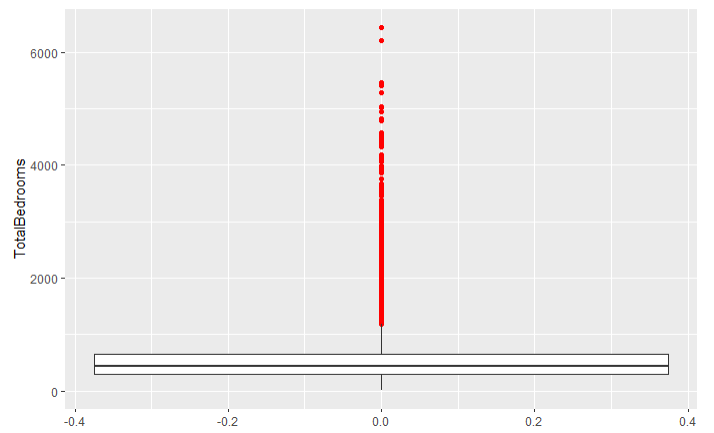
\includegraphics[width=0.7\linewidth]{figures/eda_box_5}
	\caption{Diagrama de cajas TotalBedrooms}
	\label{fig:edabox5}
\end{figure}
\newpage
\begin{figure}[h!]
	\centering
	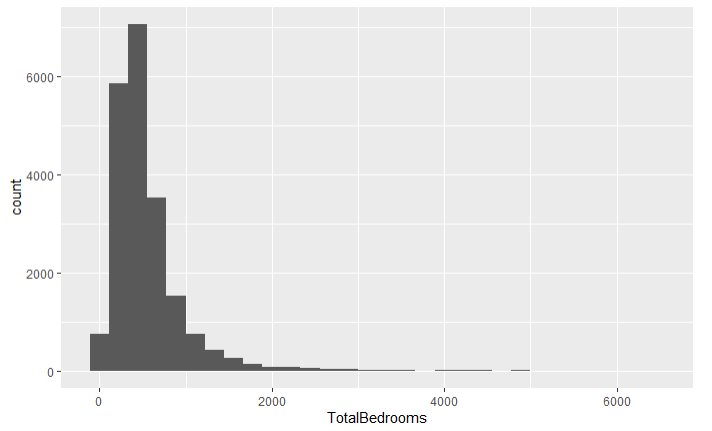
\includegraphics[width=0.7\linewidth]{figures/eda_hist_5}
	\caption{Histograma TotalBedrooms}
	\label{fig:edahist5}
\end{figure}


	
	\item \textbf{Population}: 
	\begin{table}[h!]
		\centering
		\begin{tabular}{ll}
			& Population  \\
			Valor mínimo            & 3           \\
			Primer cuartil          & 787         \\
			Mediana                 & 1166        \\
			Media                   & 1425        \\
			Tercer cuartil          & 1725        \\
			Valor máximo            & 35682       \\ \hline
			Desviación estandar     & 1132.462122 \\ \hline
			Coeficiente de skewness & 4.93549951  \\
			Coeficiente de Kurtosis & 76.535009  
		\end{tabular}
	\end{table}

Los estadísticos muestra una distribución muy estrecha, desplazada a la izquierda y con dispersión de los datos respecto de su centro, planteando la existencia de outliers.

Se complementa este estudio con la representación gráfica de esta variable mediante un diagrama de cajas y un histograma
\newpage
\begin{figure}[h!]
	\centering
	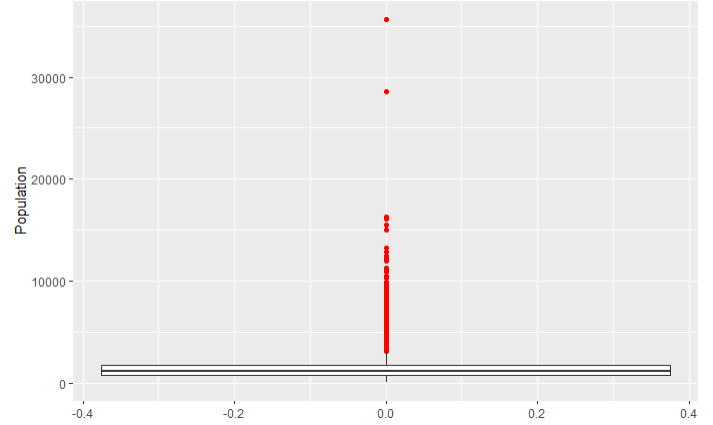
\includegraphics[width=0.7\linewidth]{figures/eda_box_6}
	\caption{Diagrama de cajas Population}
	\label{fig:edabox6}
\end{figure}
\begin{figure}[h!]
	\centering
	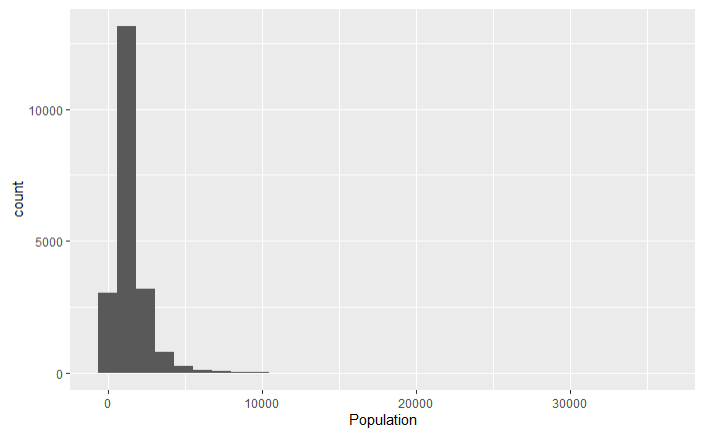
\includegraphics[width=0.7\linewidth]{figures/eda_hist_6}
	\caption{Histograma Population}
	\label{fig:edahist6}
\end{figure}

	
	\item \textbf{Households}: 
	\begin{table}[h!]
		\centering
		\begin{tabular}{ll}
			& Households \\
			Valor mínimo            & 1.0        \\
			Primer cuartil          & 280.0      \\
			Mediana                 & 409.0      \\
			Media                   & 499.5      \\
			Tercer cuartil          & 605.0      \\
			Valor máximo            & 6082.0     \\ \hline
			Desviación estandar     & 382.329753 \\ \hline
			Coeficiente de skewness & 3.41018986 \\
			Coeficiente de Kurtosis & 25.052354 
		\end{tabular}
	\end{table}

Los resultados estadísticos hacen referencia a una distribución desplazada a la izquierda con una amplia dispersión de los datos respecto al centro de distribución de estos, muy probable la existencia de outliers situados a la derecha.

Se complementa este estudio con la representación gráfica de esta variable mediante un diagrama de cajas y un histograma

\begin{figure}[h!]
	\centering
	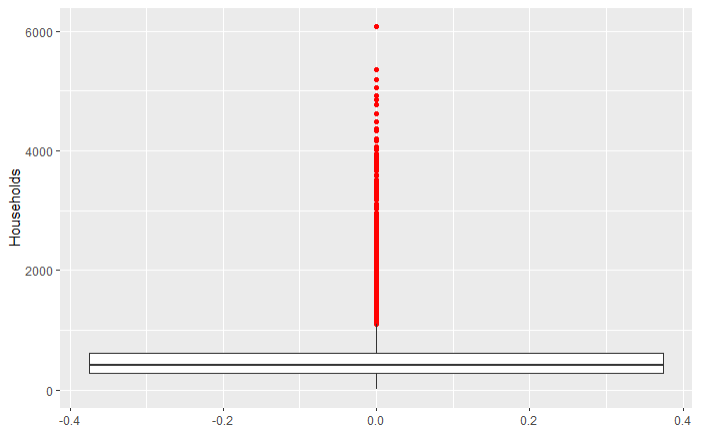
\includegraphics[width=0.7\linewidth]{figures/eda_box_7}
	\caption{Diagrama de cajas Households}
	\label{fig:edabox7}
\end{figure}
\begin{figure}[h!]
	\centering
	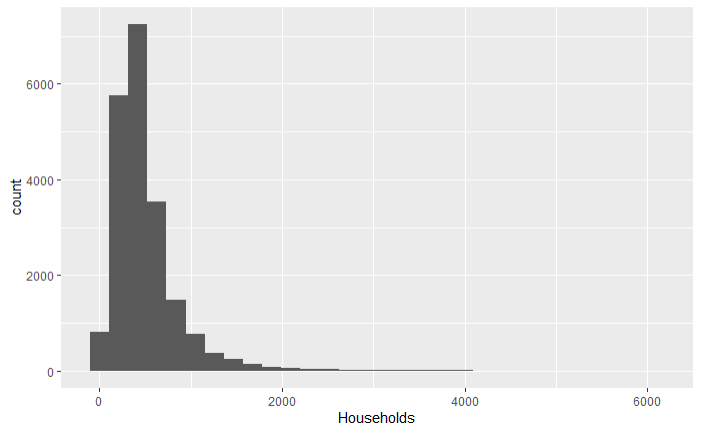
\includegraphics[width=0.7\linewidth]{figures/eda_hist_7}
	\caption{Histograma Households}
	\label{fig:edahist7}
\end{figure}

	\newpage
	\item \textbf{MedianIncome}: 
	\begin{table}[h!]
		\centering
		\begin{tabular}{ll}
			& MedianIncome \\
			Valor mínimo            & 0.4999       \\
			Primer cuartil          & 2.5634       \\
			Mediana                 & 3.5348       \\
			Media                   & 3.8707       \\
			Tercer cuartil          & 4.7432       \\
			Valor máximo            & 15.0001      \\ \hline
			Desviación estandar     & 1.899822     \\ \hline
			Coeficiente de skewness & 1.64653703   \\
			Coeficiente de Kurtosis & 7.951034    
		\end{tabular}
	\end{table}

De nuevo los datos se encuentran ligeramente desplazados a la izquierda, siendo en este caso leve la dispersión de valores respecto al centro de la distribución, revelando la existencia de outliers.

Se complementa este estudio con la representación gráfica de esta variable mediante un diagrama de cajas y un histograma

\begin{figure}[h!]
	\centering
	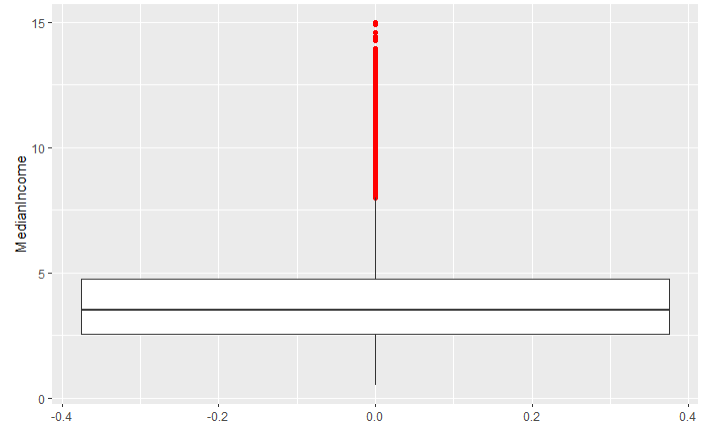
\includegraphics[width=0.7\linewidth]{figures/eda_box_8}
	\caption{Diagrama de cajas MedianIncome}
	\label{fig:edabox8}
\end{figure}
\newpage
\begin{figure}[h!]
	\centering
	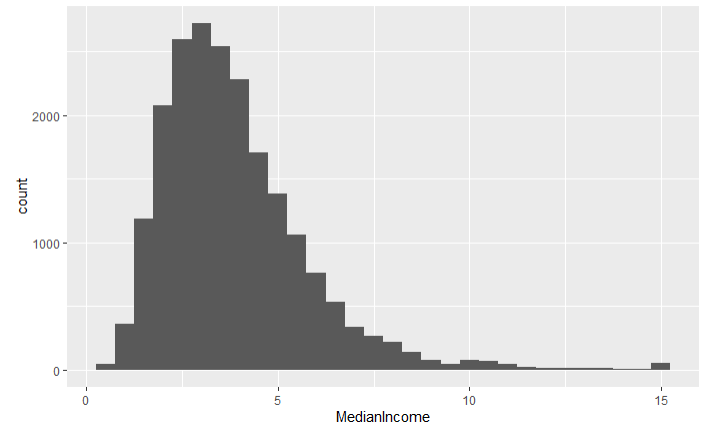
\includegraphics[width=0.7\linewidth]{figures/eda_hist_8}
	\caption{Histograma MedianIncome}
	\label{fig:edahist8}
\end{figure}


Se observa que el salario de las personas posee una distribución más o menos normal, pero con la existencia de personas con un salario más elevado que el resto, originando outliers.\\


	
\end{itemize}

Mencionar que aunque se ha indicado en cada variable que no se posee una distribución normal, esta suposición se ha confirmado realizando el test Shapiro-Wilk, el cual efectivamente no ha superado un valor por encima del nivel de significancia para ninguna de las variables, todas poseen un p-value menor a 2.2e-16. \\


Finalicemos analizando la variable dependiente, \textbf{MedianHouseValue}:
\begin{table}[h!]
	\centering
	\begin{tabular}{ll}
		& MedianHouseValue \\
		Valor mínimo            & 14999            \\
		Primer cuartil          & 119600           \\
		Mediana                 & 179700           \\
		Media                   & 206856           \\
		Tercer cuartil          & 264725           \\
		Valor máximo            & 500001           \\ \hline
		Desviación estandar     & 115395.615874    \\ \hline
		Coeficiente de skewness & 0.97769221       \\
		Coeficiente de Kurtosis & 3.327500        
	\end{tabular}
\end{table}

Se complementa este estudio con la representación gráfica de esta variable mediante un diagrama de cajas y un histograma:
\newpage

\begin{figure}[h!]
	\centering
	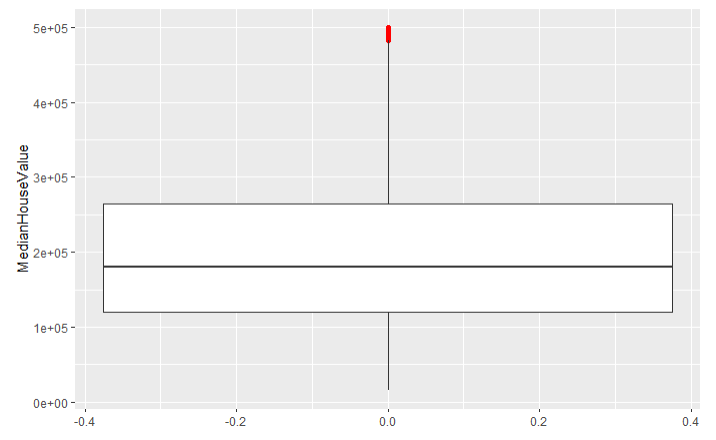
\includegraphics[width=0.7\linewidth]{figures/eda_box_9}
	\caption{Diagrama de cajas MedianHouseValue}
	\label{fig:edabox9}
\end{figure}
\begin{figure}[h!]
	\centering
	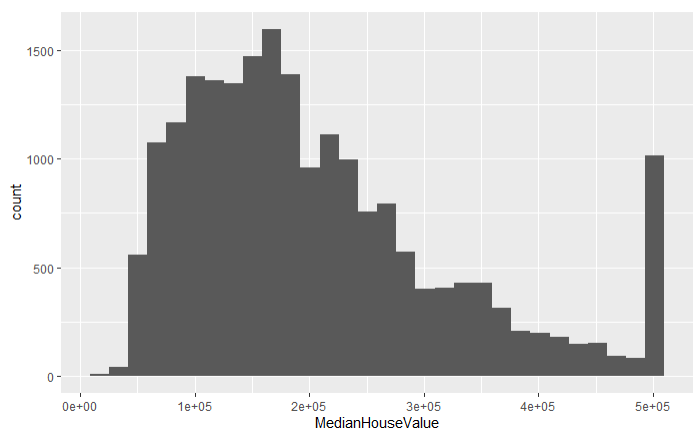
\includegraphics[width=0.7\linewidth]{figures/eda_hist_9}
	\caption{Histograma MedianHouseValue}
	\label{fig:edahist9}
\end{figure}

Se observa que la distribución de la variable dependiente posee una región central muy densa y con una leve dispersión de los datos respecto a esta. Se observa un efecto de umbral para aquellas viviendas con un valor muy elevado, ya que todas las viviendas con un valor superior a 500000 han sido fijadas en esta cantidad. \\

Comparando el valor medio de la vivienda con la media de ingresos se observa con claridad este problema:
\newpage
\begin{figure}[h!]
	\centering
	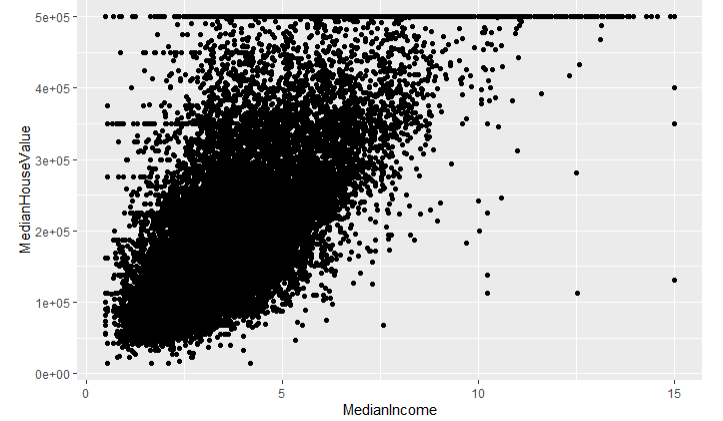
\includegraphics[width=0.7\linewidth]{figures/truncado}
	\caption{}
	\label{fig:truncado}
\end{figure}

Todos estos casos poseen un valor asignado incorrecto y por ello se procede a su eliminación, con el objetivo de evitar que estos afecten en la posterior generación de modelos. Por suerte estos casos representan un porcentaje muy bajo de los datos (sobre 1\%).

\begin{figure}[h!]
	\centering
	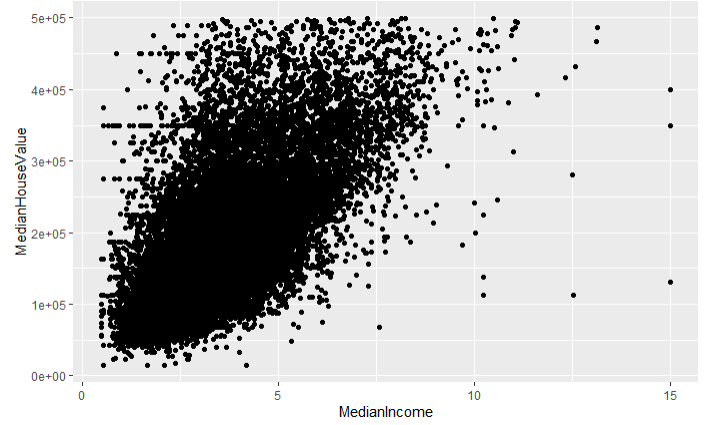
\includegraphics[width=0.7\linewidth]{figures/post-truncado}
	\caption{}
	\label{fig:post-truncado}
\end{figure}



Este paso reduce el número de outliers pero aún así se estudiaran en el siguiente apartado en aquellas variables que he considerado de estudio.

\newpage
\subsection{Análisis de valores anómalos}
Nos fijamos en los atributos anteriores en los que se presentaron valores outliers:

\begin{figure}[!tbh]
	\centering
	\begin{subfigure}{0.5\textwidth}
		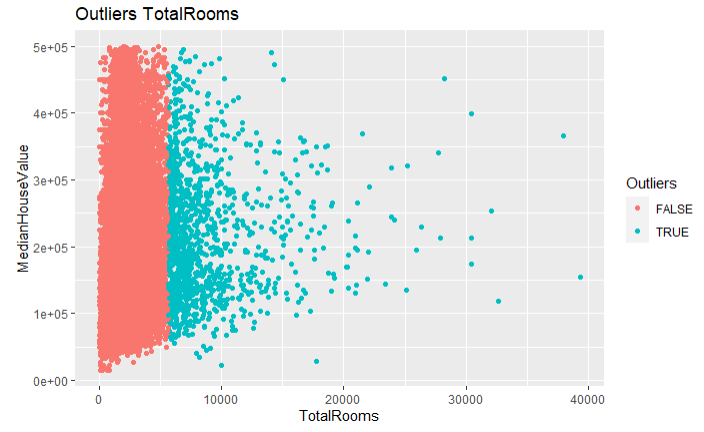
\includegraphics[width=1\linewidth]{figures/out_1}
		\caption{}
		\label{fig:out1}
	\end{subfigure}\hfil % <-- added
	\begin{subfigure}{0.5\textwidth}
		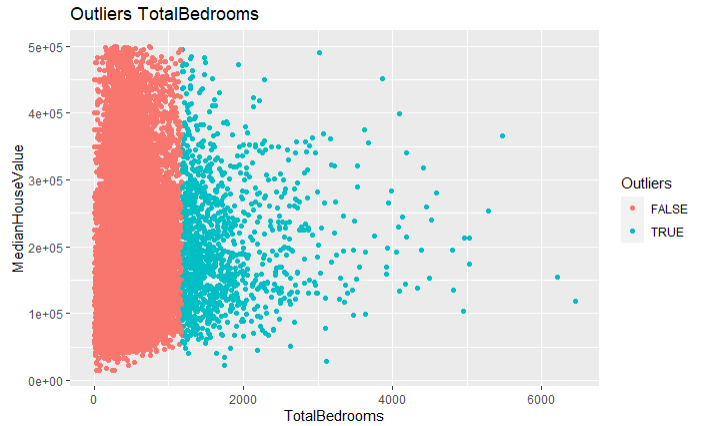
\includegraphics[width=1\linewidth]{figures/out_2}
		\caption{}
		\label{fig:out2}
	\end{subfigure}\hfil % <-- added
	
	\medskip
	
	\begin{subfigure}{0.5\textwidth}
		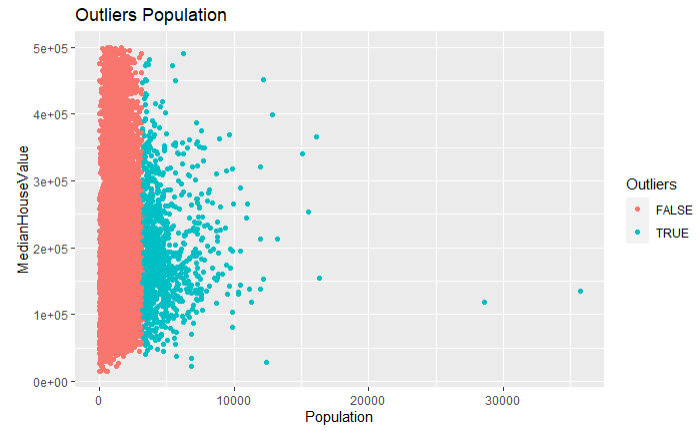
\includegraphics[width=1\linewidth]{figures/out_3}
		\caption{}
		\label{fig:out3}
	\end{subfigure}\hfil % <-- added
	\begin{subfigure}{0.5\textwidth}
		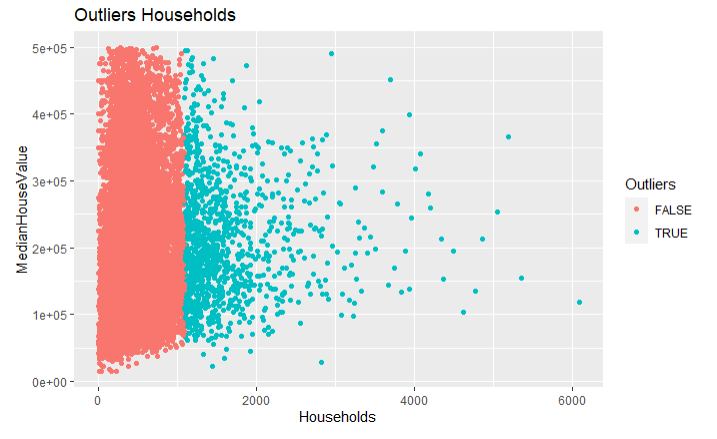
\includegraphics[width=1\linewidth]{figures/out_4}
		\caption{}
		\label{fig:out4}
	\end{subfigure}\hfil % <-- added

	\medskip
		\begin{subfigure}{0.5\textwidth}
	\centering
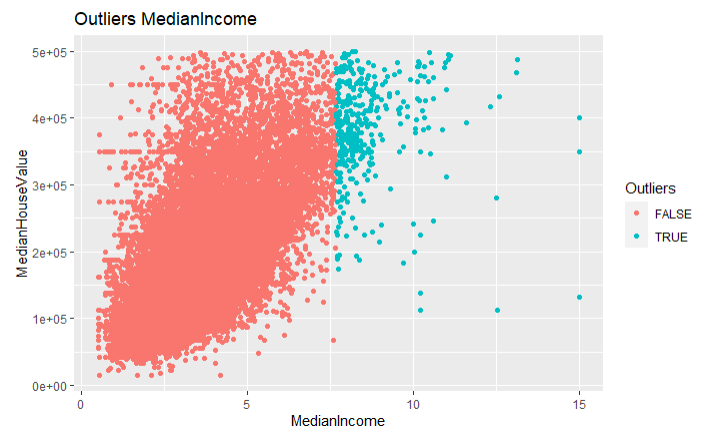
\includegraphics[width=1\linewidth]{figures/out_5}
\caption{}
\label{fig:out5}
	\end{subfigure}\hfil % <-- added
	
	\caption{Outliers California}
	\label{PCA_A}
\end{figure}





Nos fijamos solo en los casos cuyo valor del tercer cuartil más 1.5 veces su rango intercuartil, casos que son considerados como outliers extremos. Efectivamente se detectan numerosos casos que influirán de manera negativa en la realización de los modelos. Al tratarse de un 6\% del total de los datos, un porcentaje muy bajo, pues tenemos un dataset muy denso, he decidido que su eliminación será una ventaja.




\newpage
\section{Análisis de las relaciones entre variables}
Conocidas en profundidad cada una de las variables, el próximo paso es el estudio de las posibles relaciones existentes entre ellas. Este estudio tendrá como objetivo determinar si existe un alto nivel de dependencia entre algunas de las variables, detalle que debe ser tenido en cuando en el posterior proceso de elaboración de modelos.\\

El siguiente diagrama de correlaciones permite efectuar este estudio entre cada par de variables que forman el dataset. Las correlación es entre cada una de ellas s calcula gracias al test de Kendall.

\begin{figure}[h!]
	\centering
	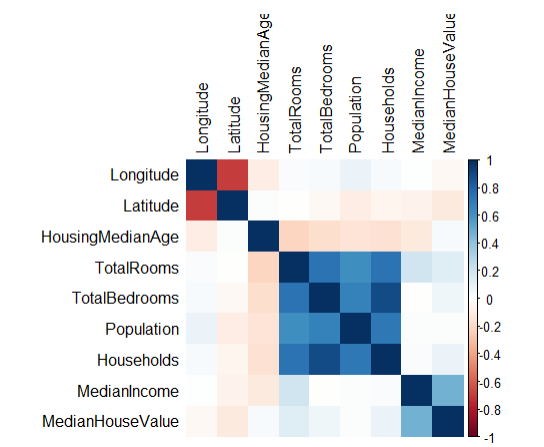
\includegraphics[width=0.7\linewidth]{figures/corre_1}
	\caption{Correlaciones California}
	\label{fig:corre1}
\end{figure}


Observando la matriz de correlación se confirman relaciones entre variables obvias y fáciles de predecir. Algunas de estas relaciones confirman que cuantos más hogares hay un bloque mayor es el número de dormitorios; de igual manera una mayor población también se vincula con un mayor número de dormitorios. Otra relación menos clara y en la que se profundiza en el siguiente apartado es en la existente relación entre la media de ingresos en el hogar con el valor medio de la vivienda.



\newpage
\section{Comprobación de hipótesis planteadas}
\textbf{California posee una amplia zona de costa permitiendo las variables de latitud y longitud determinar la cercanía de cada grupo de viviendas al mar. ¿Cómo de importante es la localización de la vivienda a la hora de determinar su precio?}

Para comprobarlo se crea un scatterplot con las variables de latitud y longitud, que utilice la variable MedianHouseValue para asignarle color a cada punto dependiendo si la media de las casas de esa zona es de un alto o bajo precio. 

\begin{figure}[h!]
	\centering
	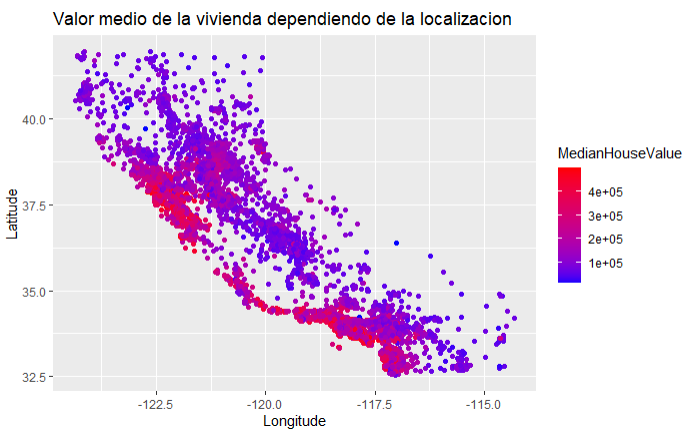
\includegraphics[width=0.7\linewidth]{figures/hipo_1}
	\caption{}
	\label{fig:hipo1}
\end{figure}

Se observa que los puntos representados pertenecen a una representación gráfica del estado de California, por ello para facilitar la compresión de los resultados se haya un mapa de este estado.

\begin{figure}[h!]
	\centering
	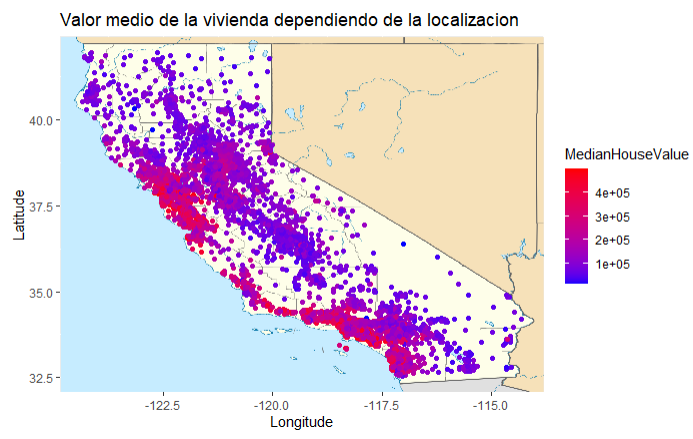
\includegraphics[width=0.7\linewidth]{figures/hipo_2}
	\caption{}
	\label{fig:hipo2}
\end{figure}

Efectivamente observamos que prácticamente todas las casas de alto valor se encuentran relativamente cerca del mar, resaltando la importancia de la proximidad a la costa en el análisis. 
Pero existe una excepción y se trata de la zona norte de California, donde a pesar de la cercanía al océano las viviendas no poseen un valor elevado. Tras investigar las diferentes ciudades de California he determinado que esto puede ser causado porque las principales ciudades de california se sitúan en la zona de costa central y sur. En la siguiente hipótesis se estudiará en más detalle esta observación.



\vspace{1cm}
\textbf{En ocasiones zonas con menos densidad de población suele estar relacionado con poblaciones más privilegiadas, ¿el precio de la vivienda tendrá una alta relación con la densidad de la población?}

De nuevo para facilitar la compresión de los resultados se efectuarán las gráficas sobre un mapa de California.


\begin{figure}[!tbh]
	\centering
	\begin{subfigure}{0.5\textwidth}
		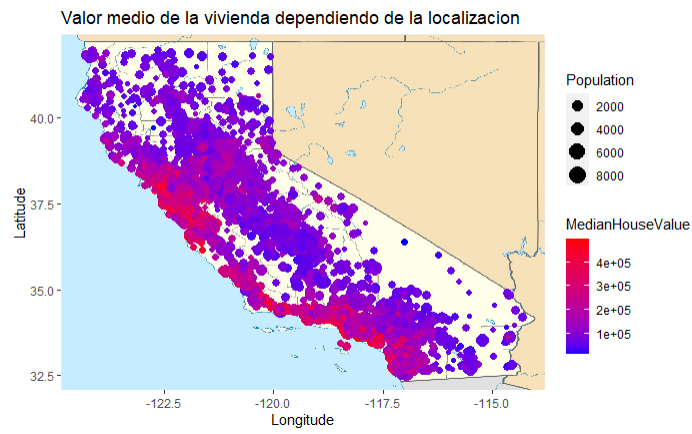
\includegraphics[width=1\linewidth]{figures/hipo_3}
		\caption{}
		\label{fig:hipo3}
	\end{subfigure}\hfil % <-- added
	\begin{subfigure}{0.5\textwidth}
		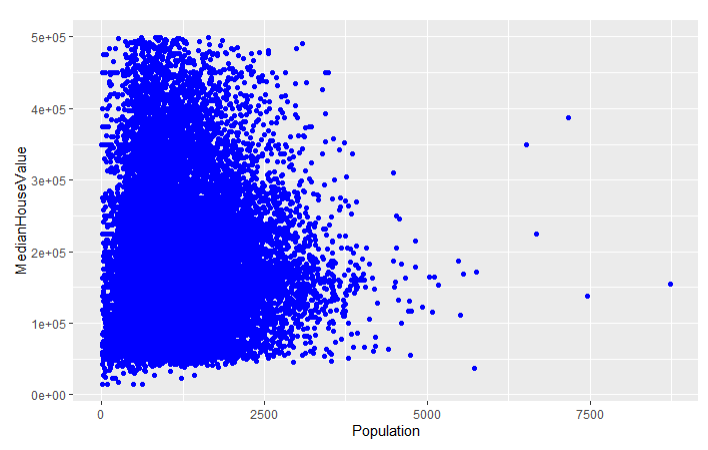
\includegraphics[width=1\linewidth]{figures/hipo_4}
		\caption{}
		\label{fig:hipo4}
	\end{subfigure}\hfil % <-- added
\end{figure}

Observamos que a pesar de que la capital de Callifornia sea Sacramento, situada en aproximadamente Latitud 38 y longitud -122, siendo una de las zonas con mayor población, la mayoría de los bloques situados en ella contienen casas de bajo presupuesto. Además se observa que cuanto más nos acercamos a regiones de montañas (centro/oeste) las poblaciones son más pequeñas al igual que el precio de la vivienda.\\

Investigando la geografía de California determino que aquellas concentraciones de viviendas de gran precio situadas en la costa corresponden a las grandes ciudades de este Estado, como son San Francisco, Los Ángeles, San Diego o San Jose. 



\newpage
\textbf{La variable MedianIncome indica los ingresos medios de los hogares, ¿posee esta una fuerte relación positiva con el valor de la vivienda?}

Nos apoyamos en un scatterplot para observar la relación entre estas dos variables.

\begin{figure}[h!]
	\centering
	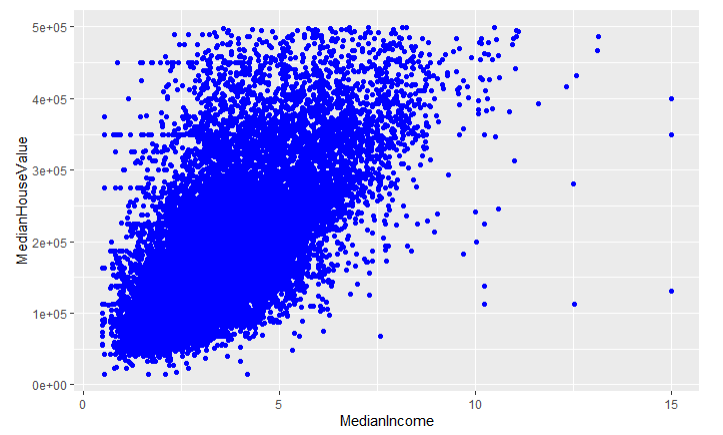
\includegraphics[width=0.7\linewidth]{figures/hipo_5}
	\caption{}
	\label{fig:hipo5}
\end{figure}

Se observa una fuerte relación entre estas variables, en la que efectivamente una media de ingresos elevados suele ir vinculada con viviendas de mayor precio. Esta relación será importante en la posterior creación de modelos de regresión.



\newpage
\textbf{Un factor interesante de estudio es la antigüedad de la vivienda, lo esperable sería que una casa nueva tuviera mayor precio que una antigua. Lo lógico es pensar que una casa nueva tenga mayor valor que una vieja.}


\begin{figure}[!tbh]
	\centering
	\begin{subfigure}{0.5\textwidth}
	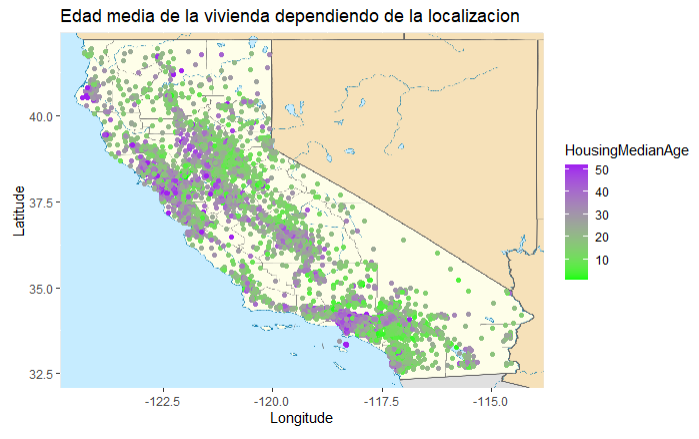
\includegraphics[width=1\linewidth]{figures/hipo_6}
\caption{}
\label{fig:hipo6}
	\end{subfigure}\hfil % <-- added
	\begin{subfigure}{0.5\textwidth}
	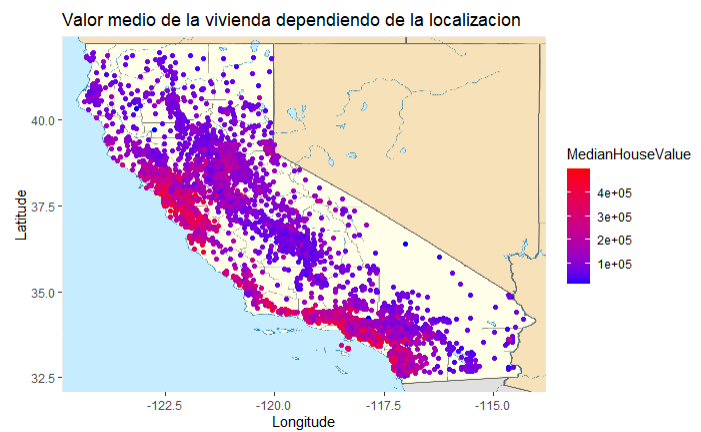
\includegraphics[width=1\linewidth]{figures/hipo_7}
\caption{}
\label{fig:hipo7}
	\end{subfigure}\hfil % <-- added
\end{figure}



Comparando los dos mapas llegamos a la conclusión de que cuanto más vieja la casa más cara es esta, algo que de primeras no parece tener sentido. Sin embargo, como ya hemos descubierto previamente, las viviendas en la costa tienen mayor precio, siendo de nuevo este el factor de mayor impacto en el dataset, junto con el ingreso de dinero en cada domicilio.\\

Podemos concluir en que cuanto más nueva sea la casa mayor será la probabilidad de que esta se ubique en una zona no costera, en el interior. 




	\newpage
	\chapter{Análisis Exploratorio de los Datos (EDA). Dataset de clasificación: Bupa}

\section{Descripción del dataset: Bupa}
El dataset \textbf{Bupa} contiene los resultados de diferentes tipos de análisis de sangre sensibles a los trastornos hepáticos que pueden surgir con un consumo excesivo de alcohol. Datos donados en el 1990.

Cada fila de este conjunto de datos contiene el registro de un solo individuo masculino.

Un dato importante de este dataset es que la séptima variable solía malinterpretarse como una variable que indica la presencia o ausencia de un trastorno hepático, pero esto es incorrecto, esta variable fue creada por investigadores para separar los datos en un conjunto de entrenamiento y otro de test.

\vspace{0.5cm}
Teniendo en cuenta la función de esta séptima variable, este dataset está formado por 5 variables independientes, las cuales corresponden a los resultados de diferentes análisis de sangre y una variable dependiente, todas variables numéricas. Se recogen un total de 345 muestras que representan el registro de cada individuo masculino.
Se presentan a continuación las variables independientes:
\begin{itemize}
	\item \textbf{mcv}: Variable numérica real que refleja el volumen corpuscular medio
	
	\item \textbf{alkphos}: Variable numérica real que refleja la fosfatasa alcalina, una enzima responsable de eliminar grupos de fosfatos de varios tipos de moléculas como nucleótidos, proteínas y otros compuestos fosforilados. Los niveles de fosfatasa alcalina elevados podrían ser signo de daño en el hígado.
	
	\item \textbf{sgpt}: Variable numérica real que refleja la alanina aminotransferasa, enzima que se encuentra principalmente en las células del hígado. Niveles altos de esta puede indicar que tiene algún tipo de daño en el hígado. 
	
	\item \textbf{sgot}: Variable numérica real que refleja la aspartato aminotransferasa, otra enzima del hígado. Los niveles elevados de esta en la sangre pueden indicar hepatitis, cirrosis, mononucleosis u otras enfermedades del hígado
	
	\item \textbf{gammagt}: Variable numérica real que refleja la gamma-glutamil transpeptidasa, es una enzima hepática. Se mide su nivel en sangre siendo un marcador de laboratorio de enfermedad hepática (mala en altos niveles).
	
	\item \textbf{selector}: Variable numérica entera creada por los investigadores para dividir los datos en el conjunto de train y test. 
\end{itemize}

La variable dependiente utilizada para la clasificación es \textbf{drinks}, un valor numérico real que refleja el número de medias pintas equivalentes a la cantidad de bebidas alcohólicas que se beben por día. 



\section{Planteamiento de hipótesis}
\begin{itemize}
	\item 
\end{itemize}





\section{Procesamiento de los datos}
Siguiendo la misma idea que con el dataset anterior se pretende profundizar en los diferentes atributos que componen este conjunto de datos para ampliar eel conocimiento sobre este y determinar cualquier característica que facilite el posterior desarrollo de modelos. \\

El primer paso es la búsqueda de missing values dentro de los datos, concluyendo en que este dataset no posee ningún Missing value.
Sin embargo se detectan 4 filas duplicadas, las cuales procedemos a eliminar, reduciéndose el número de muestras a 341.





\subsection{Análisis de las variables}
Se analiza el comportamiento de las diferentes variables mediante el calculo de diversas medidas de posición: la media aritmética, mediana, primer y tercer cuartil, valores máximos y mínimos de cada variable. También se estudia la dispersión de las distribuciones mediante el calculo  de la desviación típica, mientras que la normalidad de los datos se estudia con los coeficientes de Skewness y Kurtosis.

Se estudia cada variable en detalle mediante el calculo de las medidas previamente mencionadas. Dicho estudio es acompañado con una serie de representaciones gráficas que facilite la comprensión de los resultados:

\begin{itemize}
	\item \textbf{mcv}
	\begin{table}[]
		\begin{tabular}{ll}
			& mcv        \\
			Valor mínimo            & 65.00      \\
			Primer cuartil          & 87.00      \\
			Mediana                 & 90.00      \\
			Media                   & 90.12      \\
			Tercer cuartil          & 92.00      \\
			Valor máximo            & 103.00     \\ \hline
			Desviación estandar     & 4.4523855  \\ \hline
			Coeficiente de skewness & -0.3765269 \\
			Coeficiente de Kurtosis & 5.542126  
		\end{tabular}
	\end{table}
	
	
	\item \textbf{alkphos}: 
	\begin{table}[]
		\begin{tabular}{ll}
			& alkphos    \\
			Valor mínimo            & 23.00      \\
			Primer cuartil          & 57.00      \\
			Mediana                 & 67.00      \\
			Media                   & 69.89      \\
			Tercer cuartil          & 80.00      \\
			Valor máximo            & 138.00     \\ \hline
			Desviación estandar     & 18.4319883 \\ \hline
			Coeficiente de skewness & 0.7457300  \\
			Coeficiente de Kurtosis & 3.690844  
		\end{tabular}
	\end{table}
	
	
	\item \textbf{sgpt}: 
	\begin{table}[]
		\begin{tabular}{ll}
			& sgpt       \\
			Valor mínimo            & 4.00       \\
			Primer cuartil          & 19.00      \\
			Mediana                 & 26.00      \\
			Media                   & 30.51      \\
			Tercer cuartil          & 34.00      \\
			Valor máximo            & 155.00     \\ \hline
			Desviación estandar     & 19.5862490 \\ \hline
			Coeficiente de skewness & 3.0385262  \\
			Coeficiente de Kurtosis & 16.470290 
		\end{tabular}
	\end{table}
	
	
	\item \textbf{sgot}: 
	\begin{table}[]
		\begin{tabular}{ll}
			& sgot       \\
			Valor mínimo            & 5.00       \\
			Primer cuartil          & 19.00      \\
			Mediana                 & 23.00      \\
			Media                   & 24.66      \\
			Tercer cuartil          & 27.00      \\
			Valor máximo            & 82.00      \\ \hline
			Desviación estandar     & 10.1155409 \\ \hline
			Coeficiente de skewness & 2.2703414  \\
			Coeficiente de Kurtosis & 10.894188 
		\end{tabular}
	\end{table}
	
	
	\item \textbf{gammagt}: 
	\begin{table}[]
		\begin{tabular}{ll}
			& gammagt    \\
			Valor mínimo            & 5.0        \\
			Primer cuartil          & 15.0       \\
			Mediana                 & 25.0       \\
			Media                   & 38.4       \\
			Tercer cuartil          & 46.0       \\
			Valor máximo            & 297.0      \\ \hline
			Desviación estandar     & 39.4393786 \\ \hline
			Coeficiente de skewness & 2.8387489  \\
			Coeficiente de Kurtosis & 13.180100 
		\end{tabular}
	\end{table}
	
	
	\item \textbf{selector}: 
	Esta variable no merece de estudio profunzo pues valdrá 1 o 2 según el dato pertenezca al conjunto de entrenamiento o test.
	
	
	
	
\end{itemize}


\begin{table}[]
	\begin{tabular}{ll}
		& drinks    \\
		Valor mínimo            & 0.000     \\
		Primer cuartil          & 0.500     \\
		Mediana                 & 3.000     \\
		Media                   & 3.431     \\
		Tercer cuartil          & 5.000     \\
		Valor máximo            & 20.000    \\ \hline
		Desviación estandar     & 3.3416404 \\ \hline
		Coeficiente de skewness & 1.5616997 \\
		Coeficiente de Kurtosis & 6.673044 
	\end{tabular}
\end{table}

	\chapter{Regresión}

\section{Introducción}
Analizado el dataset 'California', en esta sección se desarrollarán diferentes modelos predictivos a partir del mismo. \\

Comenzando con el estudio y la elaboración de modelos lineales simples, posteriormente se generarán modelos más complejos, modelos no lineales y finalmente modelos basados en K-NN, todos con el objetivo explicar la variable dependiente (MedianHouseValue).




\section{Elaborar modelos lineales simples.}

Se presenta un dataset formado por más de 5 variables, por ello es necesario realizar un estudio que permita determinar aquellas 5 más relevantes.\\

Este estudio consistirá en la generación de los diferentes modelos lineales simples, con el fin de detectar aquellas variable independientes capaces de explicar un considerable porcentaje de la variable dependiente. \\

Cada modelo generado es evaluado:
\begin{table}[!h]
	\begin{tabular}{l|llll}
		Modelo Lineal                           & R\textasciicircum{}2 & R\textasciicircum{}2 Ajustado & RMSE   & p-value   \\ \hline
		MedianHouseValue $\sim$Longitude        & 0.002113             & 0.002065                      & 115300 & 3.923e-11 \\
		MedianHouseValue $\sim$Latitude         & 0.02078              & 0.02073                       & 114200 & 2.2e-16   \\
		MedianHouseValue $\sim$HousingMedianAge & 0.01116              & 0.01111                       & 114800 & 2.2e-16   \\
		MedianHouseValue $\sim$TotalRooms       & 0.018                & 0.01795                       & 114400 & 2.2e-16   \\
		MedianHouseValue $\sim$TotalBedrooms    & 0.00256              & 0.002511                      & 115300 & 3.52e-13  \\
		MedianHouseValue $\sim$Population       & 0.0006076            & 0.0005592                     & 115400 & 0.0003976 \\
		MedianHouseValue $\sim$Households       & 0.004335             & 0.004287                      & 115100 & 2.2e-16   \\
		MedianHouseValue $\sim$MedianIncome     & 0.4734               & 0.4734                        & 83740  & 2.2e-16  
	\end{tabular}
\end{table}

\newpage
Se representan gráficamente los diferentes modelos generados:

\begin{figure}[!tbh]
	\centering
	\begin{subfigure}{0.5\textwidth}
	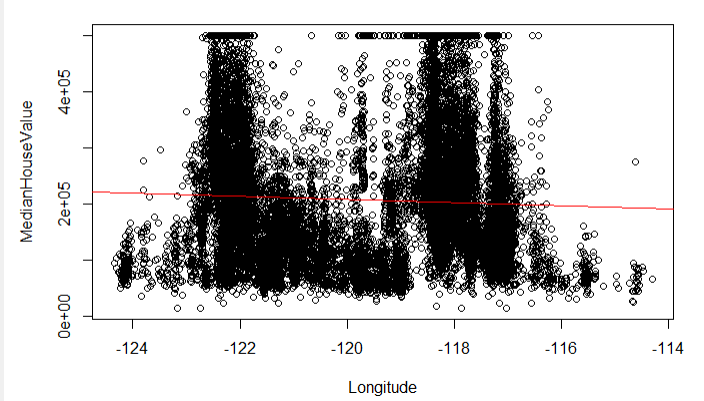
\includegraphics[width=1\linewidth]{figures/regre_1}
\caption{}
\label{fig:regre1}
	\end{subfigure}\hfil % <-- added
	\begin{subfigure}{0.5\textwidth}
	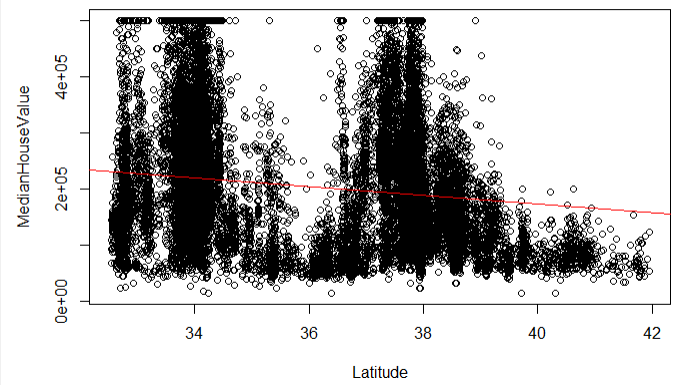
\includegraphics[width=1\linewidth]{figures/regre_2}
\caption{}
\label{fig:regre2}
	\end{subfigure}\hfil % <-- added
	
	\medskip
	
	\begin{subfigure}{0.5\textwidth}
	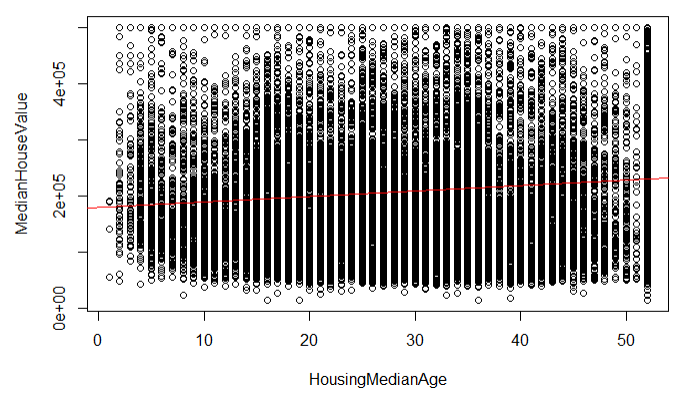
\includegraphics[width=1\linewidth]{figures/regre_3}
\caption{}
\label{fig:regre3}
	\end{subfigure}\hfil % <-- added
	\begin{subfigure}{0.5\textwidth}
	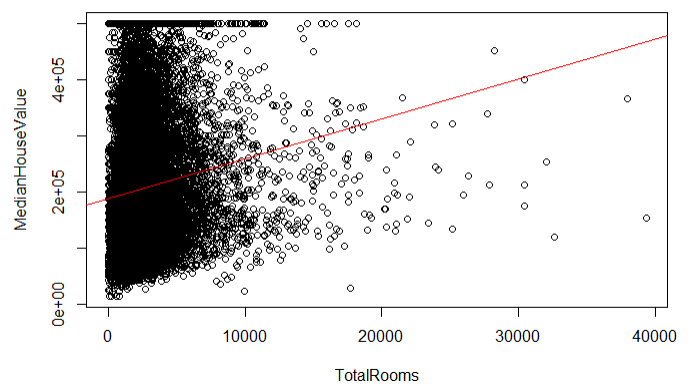
\includegraphics[width=1\linewidth]{figures/regre_4}
\caption{}
\label{fig:regre4}
	\end{subfigure}\hfil % <-- added
	
	\medskip
	
	\begin{subfigure}{0.5\textwidth}
	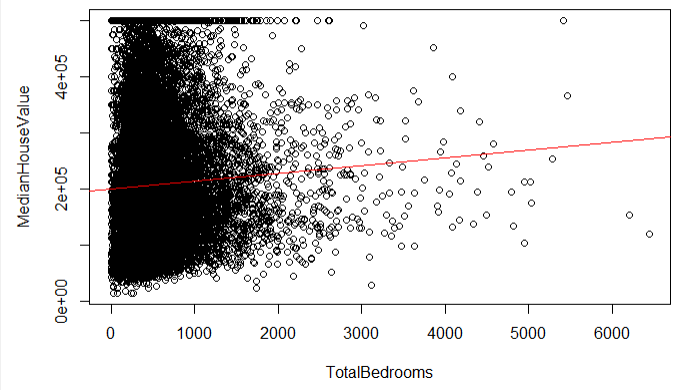
\includegraphics[width=1\linewidth]{figures/regre_5}
\caption{}
\label{fig:regre5}
	\end{subfigure}\hfil % <-- added
	\begin{subfigure}{0.5\textwidth}
	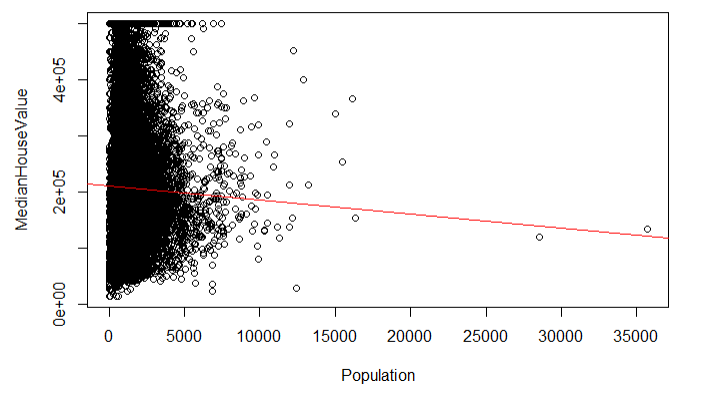
\includegraphics[width=1\linewidth]{figures/regre_6}
\caption{}
\label{fig:regre6}
	\end{subfigure}\hfil % <-- added

	\medskip

\begin{subfigure}{0.5\textwidth}
	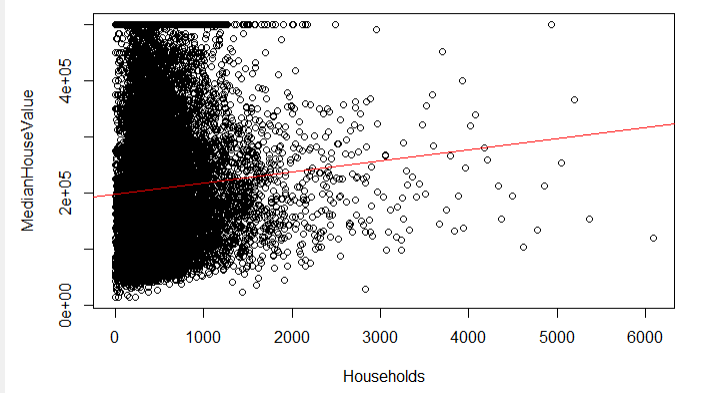
\includegraphics[width=1\linewidth]{figures/regre_7}
	\caption{}
	\label{fig:regre7}
\end{subfigure}\hfil % <-- added
\begin{subfigure}{0.5\textwidth}
	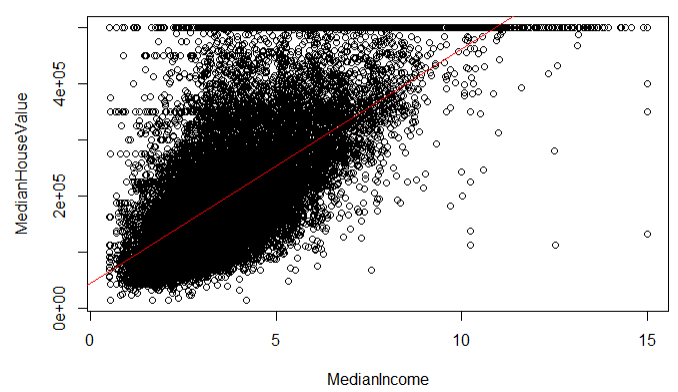
\includegraphics[width=1\linewidth]{figures/regre_8}
	\caption{}
	\label{fig:regre8}
\end{subfigure}\hfil % <-- added
	
	\caption{Modelos lineales simples}
	\label{lm}
\end{figure}





\newpage
Se observa que todos los modelos lineales generados, exceptuando el que trabaja con la variable independiente 'MedianIncome', presentan un valor de R cuadrado ajustado muy cercano a 0, lo que permite asumir que estas variable por si mismas no pueden llegar a explicar la variable dependiente 'MedianHouseValue'.\\

Fijando la atención en el caso del modelo con la variable 'MedianIncome', se presenta un valor R cuadrado ajustado próximo al 0.5, lo que se traduce en que esta variable por si sola es capaz de explicar gran parte de la variable dependiente, pero no lo suficiente. La importancia de esta variable será de utilidad para la elaboración de modelos más complejos.\\

Evaluando las métricas resultantes se observa que las 5 variables que mejor explican la variable dependiente son:
\begin{table}[!h]
	\begin{tabular}{l|llll}
		Modelo Lineal                           & R\textasciicircum{}2 & R\textasciicircum{}2 Ajustado & RMSE   & p-value \\ \hline
		MedianHouseValue $\sim$MedianIncome     & 0.4734               & 0.4734                        & 83740  & 2.2e-16 \\
		MedianHouseValue $\sim$Latitude         & 0.02078              & 0.02073                       & 114200 & 2.2e-16 \\
		MedianHouseValue $\sim$TotalRooms       & 0.018                & 0.01795                       & 114400 & 2.2e-16 \\
		MedianHouseValue $\sim$HousingMedianAge & 0.01116              & 0.01111                       & 114800 & 2.2e-16 \\
		MedianHouseValue $\sim$Households       & 0.004335             & 0.004287                      & 115100 & 2.2e-16
	\end{tabular}
\end{table}


Para finalizar este apartado se determinará cual es el mejor de estos modelos comprobando cual de ellos obtiene el menor error cuadrático medio (RMSE) en los 5 folds propuestos para este dataset.
\begin{table}[!h]
	\begin{tabular}{l|llll}
		Modelo Lineal                           & R\textasciicircum{}2 & R\textasciicircum{}2 Ajustado & RMSE   & 5-fold RMSE \\ \hline
		MedianHouseValue $\sim$MedianIncome     & 0.4734               & 0.4734                        & 83740  & 7006888908  \\
		MedianHouseValue $\sim$Latitude         & 0.02078              & 0.02073                       & 114200 & 13037618917 \\
		MedianHouseValue $\sim$TotalRooms       & 0.018                & 0.01795                       & 114400 & 13074242952 \\
		MedianHouseValue $\sim$HousingMedianAge & 0.01116              & 0.01111                       & 114800 & 13164908193 \\
		MedianHouseValue $\sim$Households       & 0.004335             & 0.004287                      & 115100 & 13256188343
	\end{tabular}
\end{table}

\vspace{0.5cm}
El modelo lineal creado en función de 'MedianIncome' ha obtenido el menor error cuadrático medio en la validación cruzada de 5-folds, confirmando de nuevo que es el mejor modelo de regresión lineal simple posible.




\newpage
\section{Elaborar modelos regresión lineal múltiple}
En este apartado se analizarán y crearán diferentes modelos que consideren varias variables independientes para explicar la variable dependiente. Para ello se procederá mediante un método descendiente, el cual consiste en partir de un modelo lineal que considere todas las posibles variables independientes y, a partir de este, se buscará la obtención de modelos progresivamente mejores mediante la eliminación de variables y/o añadiendo términos no lineales.\\

El resultado de este primer modelo es el siguiente:
\begin{figure}[!h]
	\centering
	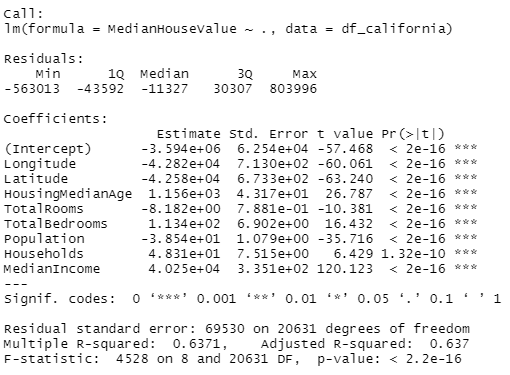
\includegraphics[width=0.7\linewidth]{figures/fit_multi1}
	\caption{}
	\label{fig:fitmulti1}
\end{figure}

Media RMSE del modelo lineal múltiple sobre 5-fold: 4844365688
\vspace{0.5cm}
\begin{table}[!h]
	\centering
	\begin{tabular}{llll}
		R\textasciicircum{}2 & R\textasciicircum{}2 Ajustado & RMSE  & 5-fold RMSE \\ \hline
		0.6371               & 0.637                         & 69530 & 4844365688 
	\end{tabular}
\end{table}

Se observa que el modelo generado ofrece mejor rendimiento frente a cualquiera de los modelos lineales simples generados en el apartado anterior. Por otro lado, los valores p-value del test de Wall no presentan valores significativos en ninguno de los casos, lo que complica la identificación de una variable de la que se pudiera prescindir.\\

Debido a esta situación, el estudio de nuevos modelos a partir de este mediante la eliminación de variables se realizará comenzando por aquellas variables que no fueron seleccionadas para el estudio de los 5 modelos lineales simples anteriores. \\

Por ello se comienza eliminando la variable independiente 'Longitude', generando el siguiente modelo:
\begin{figure}[!h]
	\centering
	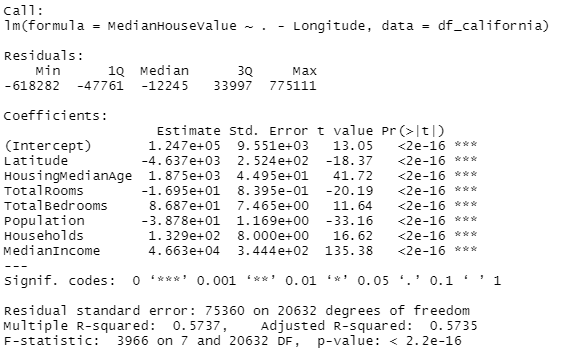
\includegraphics[width=0.7\linewidth]{figures/fit_multi_2}
	\caption{}
	\label{fig:fitmulti2}
\end{figure}

Media RMSE del modelo lineal múltiple sobre 5-fold: 5688531919
\vspace{0.5cm}
\begin{table}[!h]
	\centering
	\begin{tabular}{llll}
		R\textasciicircum{}2 & R\textasciicircum{}2 Ajustado & RMSE  & 5-fold RMSE \\ \hline
		0.5737               & 0.5735                        & 75360 & 5688531919 
	\end{tabular}
\end{table}

La eliminación de 'Longitude' da lugar a un modelo con un peor R cuadrado ajustado respecto al anterior, por ello se opta por conservar esta variable y probar eliminando la siguiente no elegida anteriormente: 'Population'.
\begin{figure}[!h]
	\centering
	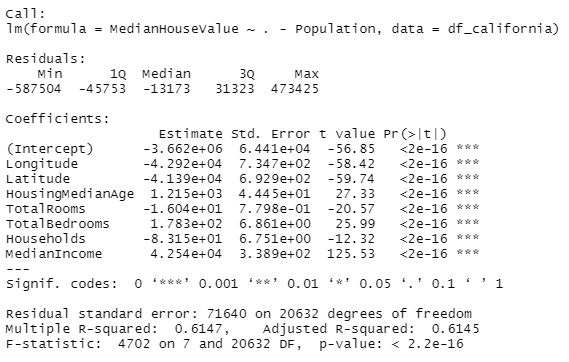
\includegraphics[width=0.7\linewidth]{figures/fit_multi_3}
	\caption{}
	\label{fig:fitmulti3}
\end{figure}

Media RMSE del modelo lineal múltiple sobre 5-fold: 5130744110
\vspace{0.5cm}
\begin{table}[!h]
	\centering
	\begin{tabular}{llll}
		R\textasciicircum{}2 & R\textasciicircum{}2 Ajustado & RMSE  & 5-fold RMSE \\ \hline
		0.6147               & 0.6145                        & 71640 & 5130744110 
	\end{tabular}
\end{table}

En este caso los resultados son levemente inferiores. Se prueba por último la eliminación de la variable 'TotalBedrooms', la última de las no elegidas entre las 5 variables más relevantes en la sección anterior.
\begin{figure}[!h]
	\centering
	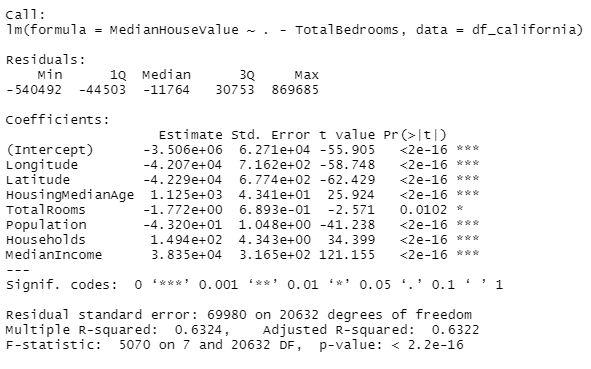
\includegraphics[width=0.7\linewidth]{figures/fit_multi_4}
	\caption{}
	\label{fig:fitmulti4}
\end{figure}

Media RMSE del modelo lineal múltiple sobre 5-fold: 4909112109
\vspace{0.5cm}
\begin{table}[!h]
	\centering
	\begin{tabular}{llll}
		R\textasciicircum{}2 & R\textasciicircum{}2 Ajustado & RMSE  & 5-fold RMSE \\ \hline
		0.6324               & 0.6322                        & 69980 & 4909112109 
	\end{tabular}
\end{table}

De nuevo los resultados son levemente peores. 
Si la eliminación de aquellas variables que no fueron seleccionada como relevantes da lugar a peores modelos podemos prácticamente deducir que con la eliminación de cada una de las 5 variables restantes los modelos obtenidos también será peores. Por ello se opta por la realización de modelos que involucren a todas las variables, pero añadiendo términos no lineales.\\

\newpage
Siendo 'MedianIncome' la variable que mejor explica la variable dependiente comencemos añadiéndola elevada al cuadrado:
\begin{figure}[!h]
	\centering
	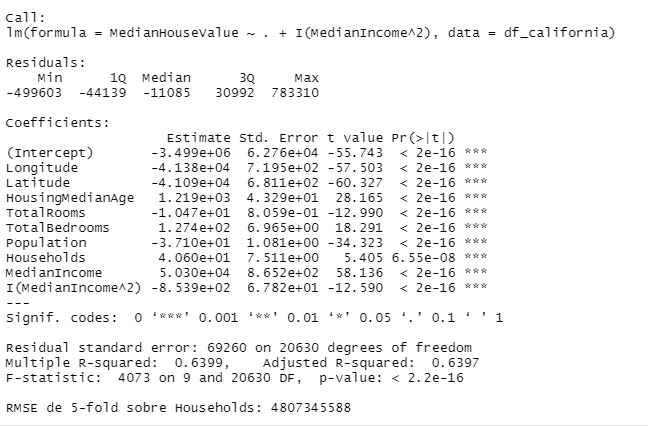
\includegraphics[width=0.7\linewidth]{figures/fit_multi_5}
	\caption{}
	\label{fig:fitmulti5}
\end{figure}

\begin{table}[!h]
	\centering
	\begin{tabular}{llll}
		R\textasciicircum{}2 & R\textasciicircum{}2 Ajustado & RMSE  & 5-fold RMSE \\ \hline
		0.6399               & 0.6397                        & 69260 & 4807345588 
	\end{tabular}
\end{table}

Se observa la generación de un modelo levemente superior respecto al formado por todas las variables.
Se prueba a continuación elevándola a 4:
\begin{figure}[!h]
	\centering
	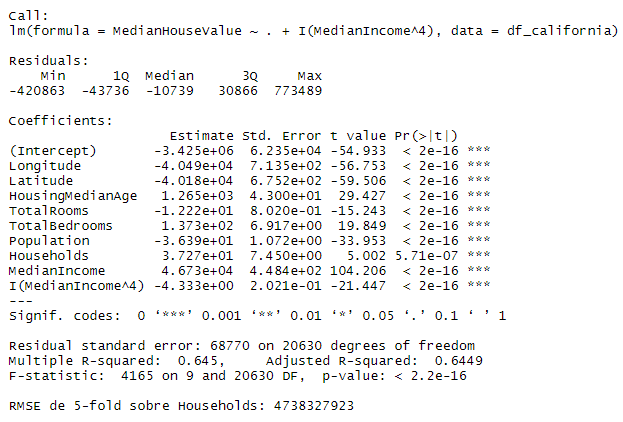
\includegraphics[width=0.7\linewidth]{figures/fit_multi_6}
	\caption{}
	\label{fig:fitmulti6}
\end{figure}

\begin{table}[!h]
	\centering
	\begin{tabular}{llll}
		R\textasciicircum{}2 & R\textasciicircum{}2 Ajustado & RMSE  & 5-fold RMSE \\ \hline
		0.645                & 0.6449                        & 68770 & 4738327923 
	\end{tabular}
\end{table}

Se produce una muy leve mejora, seguir por este camino no dará lugar a mejores resultados. 
Dado que tener en cuenta una de la variable más representativa origina modelos con mejores resultamos, añadamos el producto de las dos siguientes variables determinada como más relevante, 'Latitude' y 'TotalRooms':
\begin{figure}[!h]
	\centering
	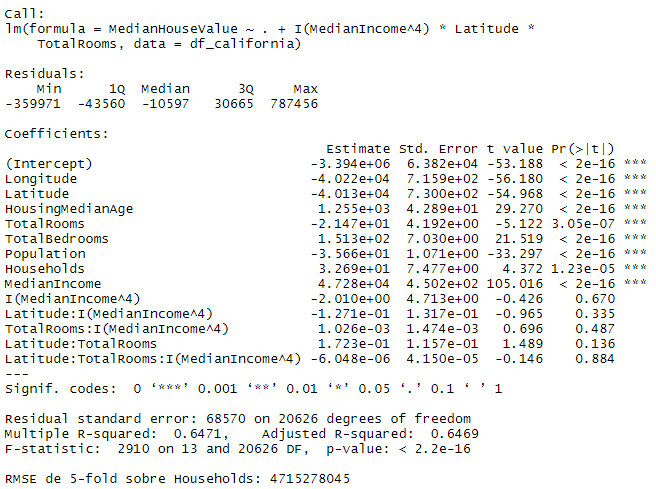
\includegraphics[width=0.7\linewidth]{figures/fit_multi_7}
	\caption{}
	\label{fig:fitmulti7}
\end{figure}

\begin{table}[!h]
	\centering
	\begin{tabular}{llll}
		R\textasciicircum{}2 & R\textasciicircum{}2 Ajustado & RMSE  & 5-fold RMSE \\ \hline
		0.6471               & 0.6469                        & 68570 & 4715278045 
	\end{tabular}
\end{table}

Se observa un modelo con unos mejores resultados, sin embargo, al observar los valores 'p-value' se desconfía de algunas variables añadidas en la multiplicación. \\

Por ello se considera en eliminar la variable 'Latitude' multiplicando.
\newpage
\begin{figure}[!h]
	\centering
	\includegraphics[width=0.7\linewidth]{figures/fit_multi_8}
	\caption{}
	\label{fig:fitmulti8}
\end{figure}

\begin{table}[!h]
	\centering
	\begin{tabular}{llll}
		R\textasciicircum{}2 & R\textasciicircum{}2 Ajustado & RMSE  & 5-fold RMSE \\ \hline
		0.6471               & 0.6469                        & 68570 & 4713390798 
	\end{tabular}
\end{table}

Efectivamente la variable 'Latitude' multiplicando no aportaba ninguna mejor.\\

Se decide continuar agregando los siguientes términos más significativos multiplicando, 'HousingMedianAge' y 'Households'
\begin{figure}[!h]
	\centering
	\includegraphics[width=0.7\linewidth]{figures/fit_multi_9}
	\caption{}
	\label{fig:fitmulti9}
\end{figure}

\begin{table}[!h]
	\centering
	\begin{tabular}{llll}
		R\textasciicircum{}2 & R\textasciicircum{}2 Ajustado & RMSE  & 5-fold RMSE \\ \hline
		0.6546               & 0.6543                        & 67850 & 4641780595 
	\end{tabular}
\end{table}

De nuevo se mejoran los resultados, pero se observa que en varios casos en los que interviene I($MedianIncome ^{4} $) aparecen valores de 'p-value' que añaden desconfianza a este término, por ello se decide probar sin elevarlo a 4.
\begin{figure}[!h]
	\centering
	\includegraphics[width=0.7\linewidth]{figures/fit_multi_10}
	\caption{}
	\label{fig:fitmulti10}
\end{figure}

\begin{table}[!h]
	\centering
	\begin{tabular}{llll}
		R\textasciicircum{}2 & R\textasciicircum{}2 Ajustado & RMSE  & 5-fold RMSE \\ \hline
		0.6594               & 0.6591                        & 67370 & 4577783319 
	\end{tabular}
\end{table}

La suposición era correcta y de nuevo han mejorado los resultados. Sin embargo, los valores *p-value* indican que no es necesaria la presencia de algunos de los términos del modelo (caso de la multiplicación de HousingMedianAge:TotalRooms:Households).\\ 

Finalmente nos quedamos con este último modelo como mejor modelo múltiple generado.








\newpage
\section{Aplicar el algoritmo k-NN para regresión}
En esta sección se elaboran y estudian modelos basados en k-NN. Este estudio se realizará sobre el mejor modelo obtenido en la sección anterior con diferentes valores de k (número de vecinos más cercanos), con el objetivo de determinar el valor de k más cercano al óptimo. \\

Por tanto la siguiente tabla recoge, para diferentes valores de k, el valor de RMSE obtenido tras realizar la validación cruzada de 5-folds, para cada caso, junto con la media de estos resultados. Utilizando en todos ellos el mejor modelo múltiple conseguido en el apartado anterior: MedianHouseValue ~ . +MedianIncome*TotalRooms*HousingMedianAge*Households.

\begin{table}[!h]
	\begin{tabular}{l|llllll}
		k  & Fold 1     & Fold 2     & Fold 3     & Fold 4     & Fold 5     & Media RMSE          \\ \hline
		5  & 4541760347 & 4530471424 & 4565272732 & 4385513226 & 4745290191 & 4553661584          \\
		7  & 4283086269 & 4381302961 & 4329091939 & 4106711363 & 4473274188 & 4314693344          \\
		10 & 4157055323 & 4196558009 & 4173551945 & 4018343901 & 4313895845 & 4171881005          \\
		20 & 4046433324 & 4096849734 & 4069779207 & 3898401005 & 4167615566 & \textbf{4051576629} \\
		25 & 4046433324 & 4096849734 & 4069779207 & 3898401005 & 4162774625 & 4054847579          \\
		50 & 4161252917 & 4184933077 & 4160816036 & 4002315397 & 4258437778 & 4153551041         
	\end{tabular}
\end{table}


Siendo la media del error RMSE obtenida en el modelo de regresión múltiple de 4577783319 sobre 5-folds, determinamos que con un k=5 ya se obtienen mejores resultados con el uso de k-NN en la validación cruzada 5-folds, siendo el valor óptimo de k un valor cercano a 20.
\begin{figure}[!h]
	\centering
	\includegraphics[width=1.2\linewidth]{figures/media}
	\caption{}
	\label{fig:media}
\end{figure}




\newpage
\section{Comparar los resultados de los dos algoritmos de regresión múltiple}
Finalmente, se comparan los resultados de los algoritmos de regresión múltiple, k-NN y, adicionalmente, el modelo M5', cuyos resultados han sido aportadas por el profesorado, ya que no ha sido tratado en el desarrollo de este proyecto.
Estas comparativas se realizan con las mismas condiciones sobre cada algoritmo, no se mantienen consideraciones específicas, se trabaja con todas las variables (MedianHouseValue ~ .).\\

En primer lugar, se utiliza el test de Wilcoxon, un test no paramétrico que permite determinar si existes relación entre dos muestras. De esta forma, se observa si existen diferencias significativas entre la regresión lineal múltiple y k-NN. La comparativa se realiza utilizando RMSE como medida de precisión para cada modelo.
Fijando el nivel de significancia en 0.05, si el p-value resultante está por debajo de este nivel, se rechaza la hipótesis nula del test, lo que indica que uno de los modelos da unos resultados significativamente distintos a los del otro modelo.

Test modelo lineal (R+) vs modelo k-NN:(R-)
\begin{table}[!h]
	\centering
	\begin{tabular}{lll}
		R+ & R- & p-value   \\ \hline
		78 & 93 & 0.7660294
	\end{tabular}
\end{table}


Puesto que el p-value resultante posee un valor superior al nivel de significancia, no es posible rechazar que ambos algoritmos ofrecen resultados similares.\\

A continuación, se utiliza el test de Friedman para determinar si existen diferencias significativas entre los 3 modelos:

Friedman rank sum test
\begin{table}[!h]
	\centering
	\begin{tabular}{lll}
		chi-squared & df & p-value \\ \hline
		8.4444      & 2  & 0.01467
	\end{tabular}
\end{table}

En este caso el valor de p-value si se sitúa por debajo del nivel de significancia, por ello se rechaza la hipótesis nula, es decir, existe al menos diferencias significativas entre un par de los algoritmos evaluados.
Finalmente aplicamos el test post-hoc de Holm para averiguar qué par es diferente y cuales se pueden considerar similares

\begin{table}[!h]
	\centering
	\begin{tabular}{l|ll}
		Modelos Regresión & Lineal Múltiple & k-NN  \\ \hline
		k-NN              & 0.580           & -     \\
		M5'               & 0.081           & 0.108
	\end{tabular}
\end{table}


Se observa la existencia de diferencias significativas entre M5' con la regresión lineal múltiple, pues su valor de p-value no superar el nivel de significancia. Los dos pares restantes poseen similitud, destacando similitud entre k-nn y regresión lineal múltiple.





	\chapter{Clasificación}

\section{Introducción}
Analizado el dataset Bupa, en este capítulo se desarrollan diferentes modelos predictivos utilizando la información obtenida previamente.
Se construirán modelos basados en k-NN (aplicado a la clasificación), modelos basados en LDA (Lineal Discriminant Analisys) y QDA (Quadratic Discriminant Analysis).\\


Importante: Tras la realización del EDA se ha optado por aplicar alguno de los cambios efectuados. Se han eliminado aquellas filas detectadas como repetidas, se ha eliminado la columna 'selector', y se han normalizado los datos.
El cambio más importante es que la variable dependiente, 'drinks', ha sido separada en dos clases tal y como se justifica en el apartado \ref{drinks}





\section{Utilizar el algoritmo k-NN probando con diferentes valores de k}
En primer lugar, se elaboran y estudian modelos de clasificación bastados en k-NN usando como métrica de rendimiento el Accuracy (precisión): la fracción de predicciones que el modelo realizó correctamente.
Se crearán diferentes modelos cada uno con un valor de k diferente.

\newpage
\begin{table}[!h]
	\resizebox{15cm}{!} {
	\begin{tabular}{l|lllllllllll}
		& Fold 1    & Fold 2    & Fold 3    & Fold 4    & Fold 5    & Fold 6    & Fold 7    & Fold 8    & Fold 9    & Fold 10   & Media     \\ \hline
		k=1  & 0.7058824 & 0.7352941 & 0.7000000 & 0.6969697 & 0.7647059 & 0.7058824 & 0.7647059 & 0.5588235 & 0.6060606 & 0.6764706 & 0.6914795 \\
		k=3  & 0.7647059 & 0.6764706 & 0.8333333 & 0.6363636 & 0.8529412 & 0.7647059 & 0.7647059 & 0.7647059 & 0.7575758 & 0.7352941 & 0.7550802 \\
		k=5  & 0.7647059 & 0.6764706 & 0.9000000 & 0.6060606 & 0.8529412 & 0.7352941 & 0.7941176 & 0.7352941 & 0.6969697 & 0.8235294 & 0.7585383 \\
		k=7  & 0.7647059 & 0.7941176 & 0.9000000 & 0.6666667 & 0.8529412 & 0.8235294 & 0.7941176 & 0.7647059 & 0.6969697 & 0.7058824 & 0.7763636 \\
		k=10 & 0.7352941 & 0.6764706 & 0.9000000 & 0.6969697 & 0.8529412 & 0.8235294 & 0.7352941 & 0.8823529 & 0.6969697 & 0.7352941 & 0.7735116 \\
		k=13 & 0.7647059 & 0.7352941 & 0.8666667 & 0.6363636 & 0.8529412 & 0.7941176 & 0.7352941 & 0.8823529 & 0.6969697 & 0.7941176 & 0.7758824 \\
		k=15 & 0.7647059 & 0.7352941 & 0.9333333 & 0.6666667 & 0.8823529 & 0.7941176 & 0.7941176 & 0.8529412 & 0.6969697 & 0.7941176 & \textbf{0.7914617} \\
		k=17 & 0.7941176 & 0.6764706 & 0.9333333 & 0.6666667 & 0.8823529 & 0.7941176 & 0.7352941 & 0.8529412 & 0.7272727 & 0.7941176 & 0.7856684 \\
		k=20 & 0.7647059 & 0.7352941 & 0.9000000 & 0.6363636 & 0.8823529 & 0.7941176 & 0.7352941 & 0.8529412 & 0.7272727 & 0.7941176 & 0.7822460 \\
		k=30 & 0.7352941 & 0.7058824 & 0.9000000 & 0.5757576 & 0.8823529 & 0.7941176 & 0.7058824 & 0.8823529 & 0.6969697 & 0.7941176 & 0.7672727
	\end{tabular}
}
\end{table}

Tras la ejecución de todos los casos, se observa que el modelo que ha obtenido el mejor rendimiento es aquel en el que el valor de k = 15, con una precisión del 79,1\%.


\vspace{1cm}
\section{Utilizar el algoritmo LDA para clasificar.}
En esta sección, se elaboran y estudian modelos de clasificacion bastados en LDA. Este tipo de modelo se realizan en base a una serie de asunciones, las cuales se deben garantizar para asegurar el correcto rendimiento del modelo.\\

La primera de estas asunciones se centra en la normalidad en las distribuciones de cada atributo. Como ya se observó durante la realización del análisis exploratorio \ref{anali}, el test de Shapiro-Wilk confirmó que no existe ninguna distribución normal dentro de los datos. \\

Otra asunción de este método es que todas las variables deben tener una varianza similar. Observemos en la siguiente tabla si es ese el caso:
\begin{table}[!h]
	\centering
	\begin{tabular}{l|l}
		Variables & Varianza     \\ \hline
		mcv       & 19.8237364   \\
		alkphos   & 339.7381922  \\
		sgpt      & 383.6211489  \\
		sgot      & 102.3241677  \\
		gammagt   & 1555.4645851
	\end{tabular}
\end{table}

Fácilmente se observa que no hay similitud entre estos valores.\\

Pese a no cumplir con las asunciones previas, se realiza el modelo LDA sin tener la garantía de correcto rendimiento del modelo. Para ello, se utiliza la función 'lda()' del paquete 'MASS'. Este método requiere especificar la variable a predecir y aquellas que se usarán para la predicción. Tanto en este caso como en el posterior modelo QDA se han utilizado todas las variables independientes para la predicción menos la variable 'selector'.

\newpage
Los resultados del modelo LDA sobre 10-folds:

\begin{table}[!h]
	\resizebox{15cm}{!} {
	\begin{tabular}{l|lllllllllll}
		& Fold 1    & Fold 2    & Fold 3    & Fold 4    & Fold 5    & Fold 6    & Fold 7    & Fold 8    & Fold 9    & Fold 10   & Media     \\ \hline
		Accuracy & 0.7058824 & 0.7352941 & 0.8666667 & 0.6363636 & 0.8235294 & 0.7941176 & 0.7058824 & 0.8823529 & 0.7575758 & 0.7941176 & 0.7701783
	\end{tabular}
}
\end{table}










\vspace{1cm}
\section{Utilizar el algoritmo QDA para clasificar.}
Finalmente, se elaboran y estudian modelos de clasificación bastados en QDA.
Respecto a las asunciones de QDA son similares a las de LDA, la única diferencia es que la similitud de las varianzas de cada variable se debe tener en cuenta respecto a cada clase a predecir. Para comprobar si se cumple, se utiliza el test de Levene:
\begin{table}[!h]
	\centering
	\begin{tabular}{l|lll}
		Variables & Df & F value & Pr(\textgreater{}F) \\ \hline
		mcv       & 1  & 0.0391  & 0.8434              \\
		alkphos   & 1  & 2.8435  & 0.09266             \\
		sgpt      & 1  & 10.646  & 0.001215            \\
		sgot      & 1  & 4.3484  & 0.03779             \\
		gammagt   & 1  & 15.386  & 0.0001061          
	\end{tabular}
\end{table}

Se observa que exceptuando el caso de la variable 'mcv', el resto no llega a un valor de p-value que supere el nivel de significancia (0.05), por lo tanto se rechaza la hipótesis nulas, confirmando que existen diferencia significativas entre las varianzas.\\

Otra de las asunciones de este modelo es la ausencia de niveles de correlación entre las distintas variables para cada clase. Se observan estos niveles de correlación mediante el coeficiente de Kendall para cada una de las dos clases:

\newpage
\begin{figure}[!tbh]
	\centering
	\begin{subfigure}{0.5\textwidth}
	\includegraphics[width=1\linewidth]{figures/corr_0}
\caption{drinks = 0}
\label{fig:corr0}
	\end{subfigure}\hfil % <-- added
	\begin{subfigure}{0.5\textwidth}
	\includegraphics[width=1\linewidth]{figures/corr_1}
\caption{drinks = 1}
\label{fig:corr1}
	\end{subfigure}\hfil % <-- added
\end{figure}



En ambos casos se observa que los niveles de correlación son bajos en prácticamente todos los casos, por lo que esta asunción si se cumple.\\

Para ejecutar QDA se utiliza la función 'qda()' de la librería 'MASS' y una vez más se utilizan todas las variables independientes para predecir la dependiente, menos la variable 'selector'. \\

Obtenemos los siguientes resultados sobre 10-folds:
\begin{table}[!h]
	\resizebox{15cm}{!} {
	\begin{tabular}{l|lllllllllll}
		& Fold 1    & Fold 2    & Fold 3    & Fold 4    & Fold 5    & Fold 6    & Fold 7    & Fold 8    & Fold 9    & Fold 10   & Media     \\ \hline
		Accuracy & 0.7352941 & 0.6764706 & 0.9000000 & 0.4848485 & 0.8235294 & 0.7941176 & 0.7058824 & 0.7941176 & 0.7272727 & 0.7647059 & 0.7406239
	\end{tabular}
}
\end{table}




\newpage
\section{Comparar los resultados de los tres algoritmos}
Los tres algoritmos han dado lugar a resultados bastantes similares, respecto al valor de precisión generado. El mejor resultado ha sido obtenido con el algoritmo knn con un número de k = 15. Justificando unos inferiores resultados con LDA se debe partir de que no se han cumplido las asunciones que acompañan a este algoritmo lo que explica el peor rendimiento de este algoritmo. De forma similar ocurre con QDA, en ambos casos se añade el factor de que no tenemos el suficiente número de casos en cada clase.

\begin{table}[!h]
	\centering
	\begin{tabular}{l|lll}
		& knn (k=15) & LDA       & QDA       \\ \hline
		Accuracy & 0.7914617  & 0.7701783 & 0.7406239
	\end{tabular}
\end{table}

Aunque se haya alcanzado una precisión superior al 70\% en todos los casos, se debe recordar que partimos de un problema balance entre el número de casos para cada una de las dos clases, lo cual se traduce en una peor clasificación la clase con menor número de casos iniciales.\\


Se finaliza con la aplicación del test de Friedman para determinar si realmente existen diferencias significativas entre los tres modelos creados. Para ello, se toman los valores de precisión resultantes para cada modelo aportado por el profesorado. En ese mismo archivo modificaremos los resultados sobre el dataset tratado, 'Bupa', para que contenga los resultados de los algoritmos efectuados a los largo de este proyecto.

Friedman rank sum test
\begin{table}[!h]
	\centering
	\begin{tabular}{lll}
		chi-squared & df & p-value \\ \hline
		0.7      & 2  & 0.7047
	\end{tabular}
\end{table}

Obteniendo un p-value superior al nivel de significancia no es posible rechazar la hipótesis nula de que los tres modelos evaluados presenten similitud entre ellos. En definitiva, se concluye en que los tres modelos generados ofrecen resultados similares sobre el conjunto de datos trabajado.














	\chapter{Apéndice}
\section{Apéndice A. Código EDA dataset de regresión 'California'}




\definecolor{miverde}{rgb}{0,0.6,0}
\definecolor{migris}{rgb}{0.5,0.5,0.5}
\definecolor{mimalva}{rgb}{0.58,0,0.82}

\lstset{ %
	backgroundcolor=\color{white},   % Indica el color de fondo; necesita que se añada \usepackage{color} o \usepackage{xcolor}
	basicstyle=\footnotesize,        % Fija el tamaño del tipo de letra utilizado para el código
	breakatwhitespace=false,         % Activarlo para que los saltos automáticos solo se apliquen en los espacios en blanco
	breaklines=true,                 % Activa el salto de línea automático
	captionpos=b,                    % Establece la posición de la leyenda del cuadro de código
	commentstyle=\color{miverde},    % Estilo de los comentarios
	deletekeywords={...},            % Si se quiere eliminar palabras clave del lenguaje
	escapeinside={\%*}{*)},          % Si quieres incorporar LaTeX dentro del propio código
	extendedchars=true,              % Permite utilizar caracteres extendidos no-ASCII; solo funciona para codificaciones de 8-bits; para UTF-8 no funciona. En xelatex necesita estar a true para que funcione.
	frame=false,	                   % Añade un marco al código
	keepspaces=true,                 % Mantiene los espacios en el texto. Es útil para mantener la indentación del código(puede necesitar columns=flexible).
	keywordstyle=\color{blue},       % estilo de las palabras clave
	language=R,                 % El lenguaje del código
	otherkeywords={*,...},           % Si se quieren añadir otras palabras clave al lenguaje
	numbers=none,                    % Posición de los números de línea (none, left, right).
	numbersep=5pt,                   % Distancia de los números de línea al código
	numberstyle=none, % Estilo para los números de línea
	rulecolor=\color{white},         % Si no se activa, el color del marco puede cambiar en los saltos de línea entre textos que sea de otro color, por ejemplo, los comentarios, que están en verde en este ejemplo
	showspaces=false,                % Si se activa, muestra los espacios con guiones bajos; sustituye a 'showstringspaces'
	showstringspaces=false,          % subraya solamente los espacios que estén en una cadena de esto
	showtabs=false,                  % muestra las tabulaciones que existan en cadenas de texto con guión bajo
	stepnumber=2,                    % Muestra solamente los números de línea que corresponden a cada salto. En este caso: 1,3,5,...
	stringstyle=\color{mimalva},     % Estilo de las cadenas de texto
	tabsize=2,	                   % Establece el salto de las tabulaciones a 2 espacios
	title=\lstname                   % muestra el nombre de los ficheros incluidos al utilizar \lstinputlisting; también se puede utilizar en el parámetro caption
}

	



\begin{lstlisting}[language=R]
#Cargo librerias necesarias
library(moments)
library(ggplot2)
library(corrplot)
library(ggpubr)
library(tidyverse)

#Cargo el dataset
california <- read.csv('california.dat', comment.char = '@', 
header = FALSE, stringsAsFactors = TRUE)

#Compruebo dimensiones e info de las variables
dim(california)
str(california)

#Pongo nombre a las variables
names(california) <- c("Longitude", "Latitude", "HousingMedianAge",
"TotalRooms", "TotalBedrooms", "Population", "Households",
"MedianIncome", "MedianHouseValue")

#Asignacion automatica, facilita el acceso a los campos
#n <- length(names(california)) - 1
#names(california)[1:n] <- paste ("X", 1:n, sep="")
#names(california)[n+1] <- "Y"

#Missing values
any(is.na(california))

#muestras duplicadas
sum(duplicated(california))

#Medidad importantes
summary(california)
desviacion = apply(california, 2, sd)
format(desviacion, scientific = FALSE)
skev <- apply(california, 2, skewness)
kurt <- apply(california, 2, kurtosis)
format(skev, scientific = FALSE)
format(kurt, scientific = FALSE)

#Representacion grafica de los diagramas de cajas
ggplot(california, aes(y=Longitude)) +
geom_boxplot(outlier.color = "red")
ggplot(california, aes(y=Latitude)) +
geom_boxplot(outlier.color = "red")
ggplot(california, aes(y=HousingMedianAge)) +
geom_boxplot(outlier.color = "red")
ggplot(california, aes(y=TotalRooms)) +
geom_boxplot(outlier.color = "red")
ggplot(california, aes(y=TotalBedrooms)) +
geom_boxplot(outlier.color = "red")
ggplot(california, aes(y=Population)) +
geom_boxplot(outlier.color = "red")
ggplot(california, aes(y=Households)) +
geom_boxplot(outlier.color = "red")
ggplot(california, aes(y=MedianIncome)) +
geom_boxplot(outlier.color = "red")

ggplot(california, aes(y=MedianHouseValue)) +
geom_boxplot(outlier.color = "red")


#Representacion grafica de los histogramas
ggplot(california, aes(x=Longitude)) +
geom_histogram()
ggplot(california, aes(x=Latitude)) +
geom_histogram()
ggplot(california, aes(x=HousingMedianAge)) +
geom_histogram()
ggplot(california, aes(x=TotalRooms)) +
geom_histogram()
ggplot(california, aes(x=TotalBedrooms)) +
geom_histogram()
ggplot(california, aes(x=Population)) +
geom_histogram()
ggplot(california, aes(x=Households)) +
geom_histogram()
ggplot(california, aes(x=MedianIncome)) +
geom_histogram()

ggplot(california, aes(x=MedianHouseValue)) +
geom_histogram()


#Test Shapiro-Wilk para comprobar normalidad en los datos
shapiro.test(sample(california[ , 'Longitude'], 5000))
shapiro.test(sample(california[ , 'Latitude'], 5000))
shapiro.test(sample(california[ , 'HousingMedianAge'], 5000))
shapiro.test(sample(california[ , 'TotalRooms'], 5000))
shapiro.test(sample(california[ , 'TotalBedrooms'], 5000))
shapiro.test(sample(california[ , 'Population'], 5000))
shapiro.test(sample(california[ , 'Households'], 5000))
shapiro.test(sample(california[ , 'MedianIncome'], 5000))


#Elimino los casos de MedianHouseValue == 500000
ggplot(california, aes(x = MedianIncome , y= MedianHouseValue)) +
geom_point()

california_clean <- drop(california[california$MedianHouseValue < 500000, ])
#Para resetear los indices
rownames(california_clean) <- NULL

ggplot(california_clean, aes(x = MedianIncome , y= MedianHouseValue)) +
geom_point()


# Estudio de los Outliers
ggplot(california_clean, aes(x = TotalRooms  , y = MedianHouseValue, color = TotalRooms > (quantile(TotalRooms, 0.75) + IQR(TotalRooms)*1.5) )) +
geom_point()  +
labs(title="Outliers TotalRooms", color="Outliers")

ggplot(california_clean, aes(x = TotalBedrooms  , y = MedianHouseValue, color = TotalBedrooms > (quantile(TotalBedrooms, 0.75) + IQR(TotalBedrooms)*1.5) )) +
geom_point()  +
labs(title="Outliers TotalBedrooms", color="Outliers")

ggplot(california_clean, aes(x = Population  , y = MedianHouseValue, color = Population > (quantile(Population, 0.75) + IQR(Population)*1.5) )) +
geom_point()  +
labs(title="Outliers Population", color="Outliers")

ggplot(california_clean, aes(x = Households  , y = MedianHouseValue, color = Households > (quantile(Households, 0.75) + IQR(Households)*1.5) )) +
geom_point()  +
labs(title="Outliers Households", color="Outliers")

ggplot(california_clean, aes(x = MedianIncome  , y = MedianHouseValue, color = MedianIncome > (quantile(MedianIncome, 0.75) + IQR(MedianIncome)*1.5) )) +
geom_point()  +
labs(title="Outliers MedianIncome", color="Outliers")


#Elimino los outliers
out_TotalRooms <- quantile(california_clean$TotalRooms, 0.75) + IQR(california_clean$TotalRooms)*1.5

out_TotalBedrooms <- quantile(california_clean$TotalBedrooms, 0.75) + IQR(california_clean$TotalBedrooms)*1.5

out_Population <- quantile(california_clean$Population, 0.75) + IQR(california_clean$Population)*1.5

out_Households <- quantile(california_clean$Households, 0.75) + IQR(california_clean$Households)*1.5



california_new <- drop(california_clean[california_clean$TotalRooms < out_TotalRooms ,])
california_new <- drop(california_clean[california_clean$TotalBedrooms < out_TotalBedrooms ,])
california_new <- drop(california_clean[california_clean$Population < out_Population ,])
california_new <- drop(california_clean[california_clean$Households < out_Households ,])
#Para resetear los indices
rownames(california_new) <- NULL

#Se eliminan un 2% solamente, interesa
dim(california_new)


#Matriz de correlaciones
corr_matrix <- cor(california_new, method = "kendall")
corrplot(corr_matrix, method = "color", tl.col = "black")


#Primera hipotesis
ggplot(california_new, aes(x = Longitude, y = Latitude, color = MedianHouseValue, hue = MedianHouseValue))+
geom_point() +
labs(title="Valor medio de la vivienda dependiendo de la localizacion", color="MedianHouseValue") +
scale_color_gradient(low="blue", high="red")

mapa <- png::readPNG("mapa.png")

ggplot(california_new, aes(x = Longitude, y = Latitude, color = MedianHouseValue, hue = MedianHouseValue))+
background_image(mapa)+
geom_point() +
labs(title="Valor medio de la vivienda dependiendo de la localizacion", color="MedianHouseValue") +
scale_color_gradient(low="blue", high="red")


#Segunda hipotesis
ggplot(california_new, aes(x = Longitude, y = Latitude, color = MedianHouseValue, size = Population))+
background_image(mapa)+
geom_point() +
labs(title="Valor medio de la vivienda dependiendo de la localizacion", color="MedianHouseValue") +
scale_color_gradient(low="blue", high="red")

ggplot(california_new, aes(x = Population, y = MedianHouseValue))+
geom_point(color = "blue") 


#Hipotesis 3
ggplot(california_new, aes(x = MedianIncome, y = MedianHouseValue))+
geom_point(color = "blue") 


#Hipotesis 4
ggplot(california_new, aes(x = HousingMedianAge, y = MedianHouseValue))+
geom_point(color = "blue") 

ggplot(california_new, aes(x = Longitude, y = Latitude, color = HousingMedianAge))+
background_image(mapa)+
geom_point() +
labs(title="Edad media de la vivienda dependiendo de la localizacion", color="HousingMedianAge") +
scale_color_gradient(low="green", high="purple")

ggplot(california_new, aes(x = Longitude, y = Latitude, color = MedianHouseValue, hue = MedianHouseValue))+
background_image(mapa)+
geom_point() +
labs(title="Valor medio de la vivienda dependiendo de la localizacion", color="MedianHouseValue") +
scale_color_gradient(low="blue", high="red")
\end{lstlisting}












	\newpage
	\section{Apéndice B. Código EDA dataset de clasificación 'Bupa'}

\begin{lstlisting}[language=R]
#Cargo librerias
library(moments)
library(ggplot2)
library(tidyverse)

#Cargo el dataset
bupa <- read.csv('bupa.dat', comment.char = '@', 
header = FALSE, stringsAsFactors = TRUE)

dim(bupa)
str(bupa)

#Asigno nombre a las variables
names(bupa) <- c("mcv", "alkphos", "sgpt",
"sgot", "gammagt", "drinks", "selector")
	
	
#Missing values
any(is.na(bupa))

#muestras duplicadas
sum(duplicated(bupa))

bupa <- bupa[!duplicated(bupa), ]
dim(bupa)

#Para resetear los indices
rownames(bupa) <- NULL

#Medidadas importantes
summary(bupa)

desviacion = apply(bupa, 2, sd)
format(desviacion, scientific = FALSE)
skev <- apply(bupa, 2, skewness)
kurt <- apply(bupa, 2, kurtosis)
format(skev, scientific = FALSE)
format(kurt, scientific = FALSE)


#Representacion grafica box_plot
ggplot(bupa, aes(y=mcv)) +
geom_boxplot(outlier.color = "red")
ggplot(bupa, aes(y=alkphos)) +
geom_boxplot(outlier.color = "red")
ggplot(bupa, aes(y=sgpt)) +
geom_boxplot(outlier.color = "red")
ggplot(bupa, aes(y=sgot)) +
geom_boxplot(outlier.color = "red")
ggplot(bupa, aes(y=gammagt)) +
geom_boxplot(outlier.color = "red")


ggplot(bupa, aes(y=drinks)) +
geom_boxplot(outlier.color = "red")



#Representacion grafica histogramas
ggplot(bupa, aes(x=mcv)) +
geom_histogram()
ggplot(bupa, aes(x=alkphos)) +
geom_histogram()
ggplot(bupa, aes(x=sgpt)) +
geom_histogram()
ggplot(bupa, aes(x=sgot)) +
geom_histogram()
ggplot(bupa, aes(x=gammagt)) +
geom_histogram()


ggplot(bupa, aes(x=drinks)) +
geom_histogram(bins = 5)


#Shapiro-wilk test
shapiro.test(sample(bupa[ , 'mcv']))
shapiro.test(sample(bupa[ , 'alkphos']))
shapiro.test(sample(bupa[ , 'sgpt']))
shapiro.test(sample(bupa[ , 'sgot']))
shapiro.test(sample(bupa[ , 'gammagt']))



#Analisis Outliers izquierda
ggplot(bupa, aes(x = mcv  , y = drinks, color = mcv < (quantile(mcv, 0.25) - IQR(mcv)*1.5) )) +
geom_point()  +
labs(title="Outliers mcv", color="Outliers")


ggplot(bupa, aes(x = sgot  , y = drinks, color = sgot < (quantile(sgot, 0.25) - IQR(sgot)*1.5) )) +
geom_point()  +
labs(title="Outliers sgot", color="Outliers")


#Analisis Outliers izquierda
ggplot(bupa, aes(x = mcv  , y = drinks, color = mcv > (quantile(mcv, 0.75) + IQR(mcv)*1.5) )) +
geom_point()  +
labs(title="Outliers mcv", color="Outliers")

ggplot(bupa, aes(x = alkphos  , y = drinks, color = alkphos > (quantile(alkphos, 0.75) + IQR(alkphos)*1.5) )) +
geom_point()  +
labs(title="Outliers alkphos", color="Outliers")

ggplot(bupa, aes(x = sgpt  , y = drinks, color = sgpt > (quantile(sgpt, 0.75) + IQR(sgpt)*1.5) )) +
geom_point()  +
labs(title="Outliers sgpt", color="Outliers")

ggplot(bupa, aes(x = sgot  , y = drinks, color = sgot > (quantile(sgot, 0.75) + IQR(sgot)*1.5) )) +
geom_point()  +
labs(title="Outliers sgot", color="Outliers")

ggplot(bupa, aes(x = gammagt  , y = drinks, color = gammagt > (quantile(gammagt, 0.75) + IQR(gammagt)*1.5) )) +
geom_point()  +
labs(title="Outliers gammagt", color="Outliers")


#Preparo la variable dependiente
unique(bupa$drinks)

bupa$drinks[bupa$drinks <= 5] <- 0
bupa$drinks[bupa$drinks > 5] <- 1

summary(bupa)



#Separo segun la variable selector
bupa_train <- bupa %>% filter(selector == 2)
bupa_test <- bupa %>% filter(selector == 1)

dim(bupa_train)
dim(bupa_test)
bupa_train %>% count(drinks)
bupa_test %>% count(drinks)


#Matriz de correlaciones
no_label_bupa <- bupa %>% select(c(-drinks, -selector))
corr_matrix <- cor(no_label_bupa, method = "kendall")
corrplot(corr_matrix, method = "num", tl.col = "black")



#Hipotesis 1
ggplot(bupa, aes(x = alkphos, y = mcv, color = drinks))+
geom_point() 

ggplot(bupa, aes(x = sgpt, y = mcv, color = drinks))+
geom_point() 

ggplot(bupa, aes(x = sgot, y = mcv, color = drinks))+
geom_point() 

ggplot(bupa, aes(x = gammagt, y = mcv, color = drinks))+
geom_point() 



#hipotesis 2
ggplot(bupa, aes(x = alkphos, y = sgpt))+
geom_point() 

ggplot(bupa, aes(x = alkphos, y = sgot))+
geom_point() 

ggplot(bupa, aes(x = alkphos, y = gammagt))+
geom_point() 


ggplot(bupa, aes(x = sgpt, y = sgot))+
geom_point() 

ggplot(bupa, aes(x = sgpt, y = gammagt))+
geom_point() 


ggplot(bupa, aes(x = sgot, y = gammagt))+
geom_point() 
\end{lstlisting}
	\newpage
	\section{Apéndice C. Código Regresión sobre California}

\begin{lstlisting}[language=R]
#Cargo librerias
library(kknn)
library(dplyr)
library(ggplot2)
library(corrplot)

#Cargo el dataset
df_california <- read.csv("california.dat", comment.char="@", header=F)

#Funcion para poner nombre a las columnas
add_colnames <- function(df) {
	colnames(df) <- c("Longitude", "Latitude", "HousingMedianAge",
	"TotalRooms", "TotalBedrooms", "Population", "Households",
	"MedianIncome", "MedianHouseValue")
	df
}

df_california <- add_colnames(df_california)


# Modelos lineales simples
lm_Longitude <- lm(MedianHouseValue ~ Longitude, data = df_california)
lm_Latitude <- lm(MedianHouseValue ~ Latitude, data = df_california)
lm_HousingMedianAge <- lm(MedianHouseValue ~ HousingMedianAge, data = df_california)
lm_TotalRooms <- lm(MedianHouseValue ~ TotalRooms, data = df_california)
lm_TotalBedrooms <- lm(MedianHouseValue ~ TotalBedrooms, data = df_california)
lm_Population <- lm(MedianHouseValue ~ Population, data = df_california)
lm_Households <- lm(MedianHouseValue ~ Households, data = df_california)
lm_MedianIncome <- lm(MedianHouseValue ~ MedianIncome, data = df_california)





summary(lm_Longitude)
summary(lm_Latitude)
summary(lm_HousingMedianAge)
summary(lm_TotalRooms)
summary(lm_TotalBedrooms)
summary(lm_Population)
summary(lm_Households)
summary(lm_MedianIncome)


#Represento graficamente los modelos
plot(MedianHouseValue ~ Longitude, data = df_california)
abline(lm_Longitude,col="red")

plot(MedianHouseValue ~ Latitude, data = df_california)
abline(lm_Latitude,col="red")

plot(MedianHouseValue ~ HousingMedianAge, data = df_california)
abline(lm_HousingMedianAge,col="red")

plot(MedianHouseValue ~ TotalRooms, data = df_california)
abline(lm_TotalRooms,col="red")

plot(MedianHouseValue ~ TotalBedrooms, data = df_california)
abline(lm_TotalBedrooms,col="red")

plot(MedianHouseValue ~ Population, data = df_california)
abline(lm_Population,col="red")

plot(MedianHouseValue ~ Households, data = df_california)
abline(lm_Households,col="red")

plot(MedianHouseValue ~ MedianIncome, data = df_california)
abline(lm_MedianIncome,col="red")



# Funcion para aplicar lm a 5-fold
run_lm_fold <- function(i, x, model, tt = "test") {
	# Cargar conjuntos de train
	file <- paste(x, "-5-", i, "tra.dat", sep="")
	x_tra <- read.csv(file, comment.char="@")
	
	# Cargar conjuntos de test
	file <- paste(x, "-5-", i, "tst.dat", sep="")
	x_tst <- read.csv(file, comment.char="@")
	
	
	
	x_tra <- add_colnames(x_tra)
	x_tst <- add_colnames(x_tst)
	
	
	if (tt == "train") {
		test <- x_tra
	} else {
		test <- x_tst
	}
	
	# Entrenar el modelo sobre el conjunto de train
	formula <- terms(model)
	model_eval <- lm(formula=formula, data=x_tra)
	
	# RMSE sobre test
	yprime <- predict(model_eval, test)
	#MSE
	sum(abs(test$MedianHouseValue - yprime)^2)/length(yprime) 
}



#Procedo a evaluar todos los modelos lineales
cat('RMSE de 5-fold sobre MedianIncome:', mean(sapply(1:5, run_lm_fold, 'california', lm_MedianIncome), fill=T))

cat('RMSE de 5-fold sobre Latitude:', mean(sapply(1:5, run_lm_fold, 'california', lm_Latitude), fill=T))

cat('RMSE de 5-fold sobre TotalRooms:', mean(sapply(1:5, run_lm_fold, 'california', lm_TotalRooms), fill=T))

cat('RMSE de 5-fold sobre HousingMedianAge:', mean(sapply(1:5, run_lm_fold, 'california', lm_HousingMedianAge), fill=T))

cat('RMSE de 5-fold sobre Households:', mean(sapply(1:5, run_lm_fold, 'california', lm_Households), fill=T))



# Modelo lineal multiple con todas las variables
fit_mult1 <- lm(MedianHouseValue ~ ., data=df_california)
summary(fit_mult1)

cat('Media RMSE del modelo lineal multiple sobre 5-fold:', mean(sapply(1:5, run_lm_fold, 'california', fit_mult1), fill=T))


#Modelo lineal multiple sin Longitude
fit_mult2 <- lm(MedianHouseValue ~ . -Longitude , data=df_california)
summary(fit_mult2)

cat('Media RMSE del modelo lineal multiple sobre 5-fold:', mean(sapply(1:5, run_lm_fold, 'california', fit_mult2), fill=T))


#Modelo lineal multiple sin Population
fit_mult3 <- lm(MedianHouseValue ~ . -Population , data=df_california)
summary(fit_mult3)

cat('Media RMSE del modelo lineal multiple sobre 5-fold:', mean(sapply(1:5, run_lm_fold, 'california', fit_mult3), fill=T))


#Modelo lineal multiple sin TotalBedrooms
fit_mult4 <- lm(MedianHouseValue ~ . -TotalBedrooms , data=df_california)
summary(fit_mult4)

cat('Media RMSE del modelo lineal multiple sobre 5-fold:', mean(sapply(1:5, run_lm_fold, 'california', fit_mult4), fill=T))


#Modelo lineal multiple MedianIncome^2
fit_mult5 <- lm(MedianHouseValue ~ . +I(MedianIncome^2) , data=df_california)
summary(fit_mult5)

cat('Media RMSE del modelo lineal multiple sobre 5-fold:', mean(sapply(1:5, run_lm_fold, 'california', fit_mult5), fill=T))

#Modelo lineal multiple MedianIncome^4
fit_mult6 <- lm(MedianHouseValue ~ . +I(MedianIncome^4) , data=df_california)
summary(fit_mult6)

cat('Media RMSE del modelo lineal multiple sobre 5-fold:', mean(sapply(1:5, run_lm_fold, 'california', fit_mult6), fill=T))

#Modelo lineal multiple I(MedianIncome^4)*Latitude*TotalRooms
fit_mult7 <- lm(MedianHouseValue ~ . +I(MedianIncome^4)*Latitude*TotalRooms , data=df_california)
summary(fit_mult7)

cat('Media RMSE del modelo lineal multiple sobre 5-fold:', mean(sapply(1:5, run_lm_fold, 'california', fit_mult7), fill=T))


#Modelo lineal multiple I(MedianIncome^4)*TotalRooms
fit_mult8 <- lm(MedianHouseValue ~ . +I(MedianIncome^4)*TotalRooms , data=df_california)
summary(fit_mult8)

cat('Media RMSE del modelo lineal multiple sobre 5-fold:', mean(sapply(1:5, run_lm_fold, 'california', fit_mult8), fill=T))


#Modelo lineal multiple I(MedianIncome^4)*TotalRooms*HousingMedianAge*Households
fit_mult9 <- lm(MedianHouseValue ~ . +I(MedianIncome^4)*TotalRooms*HousingMedianAge*Households , data=df_california)
summary(fit_mult9)

cat('Media RMSE del modelo lineal multiple sobre 5-fold:', mean(sapply(1:5, run_lm_fold, 'california', fit_mult9), fill=T))


#Modelo lineal multiple MedianIncome*TotalRooms*HousingMedianAge*Households 
fit_mult10 <- lm(MedianHouseValue ~ . +MedianIncome*TotalRooms*HousingMedianAge*Households , data=df_california)
summary(fit_mult10)

cat('Media RMSE del modelo lineal multiple sobre 5-fold:', mean(sapply(1:5, run_lm_fold, 'california', fit_mult10), fill=T))



#Funcion para aplicar knn sobre 5-folds
run_knn_fold <- function(i, x, formula, k,  tt = "test") {
	# Cargar conjuntos de train
	file <- paste(x, "-5-", i, "tra.dat", sep="")
	x_tra <- read.csv(file, comment.char="@")
	
	# Cargar conjuntos de test
	file <- paste(x, "-5-", i, "tst.dat", sep="")
	x_tst <- read.csv(file, comment.char="@")
	
	
	
	x_tra <- add_colnames(x_tra)
	x_tst <- add_colnames(x_tst)
	
	
	if (tt == "train") {
		test <- x_tra
	} else {
		test <- x_tst
	}
	
	# Entrenar el modelo sobre el conjunto de train
	model_eval <- kknn(formula=formula, x_tra, test, k=k)
	
	# RMSE sobre test
	yprime <- model_eval$fitted.values
	#MSE
	sum(abs(test$MedianHouseValue - yprime)^2)/length(yprime) 
}


#Pruebo con diferentes valores de k
cat('RMSE del modelo k-NN sobre 5-fold:', sapply(1:5, run_knn_fold, 'california', MedianHouseValue ~ . +MedianIncome*TotalRooms*HousingMedianAge*Households, k = 5), fill=T)
cat('Meida RMSE del modelo k-NN sobre 5-fold:', mean(sapply(1:5, run_knn_fold, 'california', MedianHouseValue ~ . +MedianIncome*TotalRooms*HousingMedianAge*Households, k = 5), fill=T))


cat('RMSE del modelo k-NN sobre 5-fold:', sapply(1:5, run_knn_fold, 'california', MedianHouseValue ~ . +MedianIncome*TotalRooms*HousingMedianAge*Households, k = 7), fill=T)
cat('Meida RMSE del modelo k-NN sobre 5-fold:', mean(sapply(1:5, run_knn_fold, 'california', MedianHouseValue ~ . +MedianIncome*TotalRooms*HousingMedianAge*Households, k = 7), fill=T))


cat('RMSE del modelo k-NN sobre 5-fold:', sapply(1:5, run_knn_fold, 'california', MedianHouseValue ~ . +MedianIncome*TotalRooms*HousingMedianAge*Households, k = 10), fill=T)
cat('Meida RMSE del modelo k-NN sobre 5-fold:', mean(sapply(1:5, run_knn_fold, 'california', MedianHouseValue ~ . +MedianIncome*TotalRooms*HousingMedianAge*Households, k = 10), fill=T))


cat('RMSE del modelo k-NN sobre 5-fold:', sapply(1:5, run_knn_fold, 'california', MedianHouseValue ~ . +MedianIncome*TotalRooms*HousingMedianAge*Households, k = 20), fill=T)
cat('Meida RMSE del modelo k-NN sobre 5-fold:', mean(sapply(1:5, run_knn_fold, 'california', MedianHouseValue ~ . +MedianIncome*TotalRooms*HousingMedianAge*Households, k = 20), fill=T))


cat('RMSE del modelo k-NN sobre 5-fold:', sapply(1:5, run_knn_fold, 'california', MedianHouseValue ~ . +MedianIncome*TotalRooms*HousingMedianAge*Households, k = 25), fill=T)
cat('Meida RMSE del modelo k-NN sobre 5-fold:', mean(sapply(1:5, run_knn_fold, 'california', MedianHouseValue ~ . +MedianIncome*TotalRooms*HousingMedianAge*Households, k = 25), fill=T))


cat('RMSE del modelo k-NN sobre 5-fold:', sapply(1:5, run_knn_fold, 'california', MedianHouseValue ~ . +MedianIncome*TotalRooms*HousingMedianAge*Households, k = 50), fill=T)
cat('Meida RMSE del modelo k-NN sobre 5-fold:', mean(sapply(1:5, run_knn_fold, 'california', MedianHouseValue ~ . +MedianIncome*TotalRooms*HousingMedianAge*Households, k = 50), fill=T))


#knn sobre modelo con todas las variables
cat('RMSE del modelo k-NN sobre 5-fold:', sapply(1:5, run_knn_fold, 'california', MedianHouseValue ~ ., k = 20), fill=T)
cat('Meida RMSE del modelo k-NN sobre 5-fold:', mean(sapply(1:5, run_knn_fold, 'california', MedianHouseValue ~ ., k = 20), fill=T))




# Comparativa LM, k-NN y M5'
#leemos la tabla con los errores medios de test
resultados <- read.csv("regr_test_alumnos.csv")
tablatst <- cbind(resultados[,2:dim(resultados)[2]])
colnames(tablatst) <- names(resultados)[2:dim(resultados)[2]]
rownames(tablatst) <- resultados[,1]


#Calculo mis valores de LM y KNN para aniadirlos en la tabla
media_lm <-mean(sapply(1:5, run_lm_fold, 'california', fit_mult1), fill=T)
media_knn <- mean(sapply(1:5, run_knn_fold, 'california', MedianHouseValue ~., k = 20), fill=T)

tablatst["california", 1] <- media_lm
tablatst["california", 2] <- media_knn

#Comparar lm con knn con Wilcoxon
# + 0.1 porque wilcox R falla para valores == 0 en la tabla
difs <- (tablatst[,1] - tablatst[,2]) / tablatst[,1]
wilc_1_2 <- cbind(ifelse (difs<0, abs(difs)+0.1, 0+0.1),
ifelse (difs>0, abs(difs)+0.1, 0+0.1))

colnames(wilc_1_2) <- c(colnames(tablatst)[1], colnames(tablatst)[2])
head(wilc_1_2)

LMvsKNNtst <- wilcox.test(wilc_1_2[,1], wilc_1_2[,2], alternative = "two.sided", paired=TRUE)
Rmas <- LMvsKNNtst$statistic
pvalue <- LMvsKNNtst$p.value

LMvsKNNtst <- wilcox.test(wilc_1_2[,2], wilc_1_2[,1], alternative = "two.sided", paired=TRUE)
Rmenos <- LMvsKNNtst$statistic


cat('Test modelo lineal (R+) vs modelo k-NN:(R-)', fill=T)
cat('Valor R+: ',Rmas, fill=T)
cat('Valor R-: ',Rmenos, fill=T)
cat('p-value del test: ',pvalue, fill=T)


test_friedman <- friedman.test(as.matrix(tablatst))
test_friedman

tam <- dim(tablatst)
groups <- rep(1:tam[2], each=tam[1])
pairwise.wilcox.test(as.matrix(tablatst), groups, p.adjust = "holm", paired = TRUE)
\end{lstlisting}
	\newpage
	\section{Apéndice D. Código Clasificación sobre Bupa}

\begin{lstlisting}[language=R]
#Cargo librerias
library(tidyverse)
library(class)
library(caret)
library(car)
library("MASS")
library(corrplot)


#Cargo el dataset
bupa <- read.csv('bupa.dat', comment.char = '@', 
header = FALSE, stringsAsFactors = TRUE)

dim(bupa)
str(bupa)

#asigno nombre a las variables
names(bupa) <- c("mcv", "alkphos", "sgpt",
"sgot", "gammagt", "drinks", "selector")


#Elimino casos duplicados
bupa <- bupa[!duplicated(bupa), ]

#Para resetear los indices
rownames(bupa) <- NULL

#Defino unicamente dos clases en la variable dependiente drinks
unique(bupa$drinks)
bupa$drinks[bupa$drinks <= 5] <- 0
bupa$drinks[bupa$drinks > 5] <- 1
	
	
	
#Separo segun la variable selector
bupa_train <- bupa %>% filter(selector == 2)
bupa_test <- bupa %>% filter(selector == 1)

bupa_train <- bupa_train %>% select(-selector)
bupa_test <- bupa_test %>% select(-selector)


summary(bupa_train)


#Normalizo los datos, la variable dependiente no
bupa_train_scale <- as.data.frame(scale(bupa_train))
bupa_train_scale[,'drinks'] <- bupa_train$drinks
bupa_test_scale <- as.data.frame(scale(bupa_test))
bupa_test_scale[,'drinks'] <- bupa_test$drinks


# Modelo con k=7
knn_pred_1 <- knn(train=bupa_train_scale[,-ncol(bupa_train_scale)],                                                  test=bupa_test_scale[,-ncol(bupa_test_scale)],
cl=bupa_train_scale[,ncol(bupa_train_scale)], k=7)

# Evaluo los resultados del modelo creado
result <- table(knn_pred_1, bupa_test_scale[, 'drinks'])

# Precision obtenida
sum(diag(result)) / length(knn_pred_1)



# Modelos basados en k-NN
#Cargo todos los modelos pues debo aplicar los cambios
# Cargar conjuntos de entrenamiento
bupa_train1 <- read.csv("bupa-10-1tra.dat", comment.char="@")
bupa_train2 <- read.csv("bupa-10-2tra.dat", comment.char="@")
bupa_train3 <- read.csv("bupa-10-3tra.dat", comment.char="@")
bupa_train4 <- read.csv("bupa-10-4tra.dat", comment.char="@")
bupa_train5 <- read.csv("bupa-10-5tra.dat", comment.char="@")
bupa_train6 <- read.csv("bupa-10-6tra.dat", comment.char="@")
bupa_train7 <- read.csv("bupa-10-7tra.dat", comment.char="@")
bupa_train8 <- read.csv("bupa-10-8tra.dat", comment.char="@")
bupa_train9 <- read.csv("bupa-10-9tra.dat", comment.char="@")
bupa_train10 <- read.csv("bupa-10-10tra.dat", comment.char="@")

# Cargar conjuntos de test
bupa_test1 <- read.csv("bupa-10-1tst.dat", comment.char="@")
bupa_test2 <- read.csv("bupa-10-2tst.dat", comment.char="@")
bupa_test3 <- read.csv("bupa-10-3tst.dat", comment.char="@")
bupa_test4 <- read.csv("bupa-10-4tst.dat", comment.char="@")
bupa_test5 <- read.csv("bupa-10-5tst.dat", comment.char="@")
bupa_test6 <- read.csv("bupa-10-6tst.dat", comment.char="@")
bupa_test7 <- read.csv("bupa-10-7tst.dat", comment.char="@")
bupa_test8 <- read.csv("bupa-10-8tst.dat", comment.char="@")
bupa_test9 <- read.csv("bupa-10-9tst.dat", comment.char="@")
bupa_test10 <- read.csv("bupa-10-10tst.dat", comment.char="@")


#Funcion para hacer las transformaciones del EDA en todos los folds
df_prepare <- function(df){
	names(df) <- c("mcv", "alkphos", "sgpt",
	"sgot", "gammagt", "drinks", "selector")
	
	#eliminar repetidos
	df <- df[!duplicated(df), ]
	#Para resetear los indices
	rownames(df) <- NULL
	
	#Eliminados la columna selector, no es util
	df <- df %>% select(-selector)
	
	df$drinks[df$drinks <= 5] <- 0
	df$drinks[df$drinks > 5] <- 1
	
	df_scale <- as.data.frame(scale(df))
	df_scale[,'drinks'] <- df$drinks
	
	df_scale
}



# Generamos listas que contienen los folds de Validacion Cruzada.
train_list <- list(bupa_train1, bupa_train2, bupa_train3, bupa_train4, bupa_train5, bupa_train6, bupa_train7, bupa_train8, bupa_train9, bupa_train10)

test_list <- list(bupa_test1, bupa_test2, bupa_test3, bupa_test4, bupa_test5, bupa_test6, bupa_test7, bupa_test8, bupa_test9, bupa_test10)


#Aplicamos los cambios en todos
train_list <- lapply(train_list, df_prepare)
test_list <- lapply(test_list, df_prepare)




# Evaluar modelos con validacion cruzada 10-fold
knn_fold_bupa <- function(train_list, test_list, k) {
	sapply(1:length(train_list), function(i) {
		# Aplicamos modelo
		pred <- knn(train = train_list[[i]] %>% select(-drinks), 
		test = test_list[[i]] %>% select(-drinks), 
		cl = train_list[[i]]$drinks, k=k)
		# Calculamos el accuracy
		sum(pred == test_list[[i]]$drinks) / length(pred)
	})
}

# Evaluar knn train con diferentes k
knn_1 <- knn_fold_bupa(train_list, test_list, 1)
knn_2 <- knn_fold_bupa(train_list, test_list, 3)
knn_3 <- knn_fold_bupa(train_list, test_list, 5)
knn_4 <- knn_fold_bupa(train_list, test_list, 7)
knn_5 <- knn_fold_bupa(train_list, test_list, 10)
knn_6 <- knn_fold_bupa(train_list, test_list, 13)
knn_7 <- knn_fold_bupa(train_list, test_list, 15)
knn_8 <- knn_fold_bupa(train_list, test_list, 17)
knn_9 <- knn_fold_bupa(train_list, test_list, 20)
knn_10 <- knn_fold_bupa(train_list, test_list, 30)

#Agrupo los resultados en una tabla
l <- rbind(knn_1, knn_2, knn_3, knn_4, knn_5, knn_6, knn_7, knn_8, knn_9, knn_10)
l_mean <- cbind(apply(l, 1, mean))
l_all <- cbind(l, apply(l, 1, mean))


# Knn en train del mejor modelo
knn_7 <- knn_fold_bupa(train_list, test_list, 15)
mean(knn_7)



# Comprobamos variabilidad para LDA
var_test <- apply(bupa, 2, var)
var_test


# Funcion para LDA en validacion cruzada
lda_fold_bupa <- function(formula, train_list, test_list) {
	sapply(1:length(train_list), function(i) {
		# modelo lda
		fit <- lda(formula, data = train_list[[i]])
		# Calculamos predicciones
		pred <- predict(fit, test_list[[i]]%>%select(-drinks))
		
		# Calculamos la precision
		sum(pred$class == test_list[[i]]$drinks) / length(pred$class)
	})
}


#Aplico lda
lda_fold <- lda_fold_bupa(drinks ~ ., train_list, test_list)

mean(lda_fold)



# Comprobamos variabilidad para QDA
#Cambio para poder usar levene test
bupa$drinks[bupa$drinks == 0] <- '0'
bupa$drinks[bupa$drinks == 1] <- '1'

leveneTest(mcv ~ drinks, bupa)
leveneTest(alkphos ~ drinks, bupa)
leveneTest(sgpt ~ drinks, bupa)
leveneTest(sgot ~ drinks, bupa)
leveneTest(gammagt ~ drinks, bupa)

bupa$drinks[bupa$drinks == 0] <- 0
bupa$drinks[bupa$drinks == 1] <- 1

#Correlacion por clases
bupa_0 <- bupa %>% filter(drinks == 0) %>% select(-c(selector,drinks))

corr_matrix <- cor(bupa_0, method = "kendall")
corrplot(corr_matrix, method = "num", tl.col = "black")

bupa_1 <- bupa %>% filter(drinks == 1) %>% select(-c(selector,drinks))

corr_matrix <- cor(bupa_1, method = "kendall")
corrplot(corr_matrix, method = "num", tl.col = "black")




# Funcion para QDA en validacion cruzada
qda_fold_bupa <- function(formula, train_list, test_list) {
	sapply(1:length(train_list), function(i) {
		# modelo lda
		fit <- qda(formula, data = train_list[[i]])
		# Calculamos predicciones
		pred <- predict(fit, test_list[[i]]%>%select(-drinks))
		
		# Calculamos la precision
		sum(pred$class == test_list[[i]]$drinks) / length(pred$class)
	})
}

qda_fold <- qda_fold_bupa(drinks ~ ., train_list, test_list)
mean(qda_fold)


#Agrupamos los resultados de los 3 modelos
results <- cbind(mean(knn_7), mean(lda_fold), mean(qda_fold))
results

#leemos la tabla con los errores medios de test
resultados <- read.csv("clasif_test_alumos.csv")
tablatst <- cbind(resultados[,2:dim(resultados)[2]])
colnames(tablatst) <- names(resultados)[2:dim(resultados)[2]]
rownames(tablatst) <- resultados[,1]

#Pongo mis resultados en mi dataset bupa
tablatst["bupa", ] <- results

# test friedman
test_friedman <- friedman.test(as.matrix(tablatst))
test_friedman
\end{lstlisting}
	\newpage
	
	
	
	\addcontentsline{toc}{chapter}{Referencias Bibliográficas}
	
	\bibliographystyle{ieeetr}
	\bibliography{references}
	
	
	
	
	
	
\end{document}